\documentclass[a4paper,twoside]{bth}
\newcommand{\thesisDegree}{Master of Science in Software Engineering}
\newcommand{\thesisMonth}{May}
\newcommand{\thesisYear}{2026}
\newcommand{\faculty}{Computing}
\newcommand{\thesisWeeks}{20}
\newcommand{\thesisTitle}{Human-AI Collaboration for Decision-Making in Agile Sprint Planning}
\newcommand{\thesisSubtitle}{A Practitioner-Informed Conceptual Model}
\newcommand{\authorFirst}{Ungarala Sai Krishna Yashwanth}
\newcommand{\authorFirstMail}{saun24@student.bth.se}
\newcommand{\authorSecond}{Mihir Singh Thakur}
\newcommand{\authorSecondMail}{mith24@student.bth.se}
\newcommand{\super}{Henry Edison, PhD}
\newcommand{\superAffiliation}{Software Engineering}

\usepackage[utf8]{inputenc}
\usepackage[T1]{fontenc}
\usepackage{graphicx}
\usepackage{amsmath}
\usepackage{amssymb}
\usepackage{textcomp}
\usepackage{longtable}
\usepackage{multirow}
\usepackage{booktabs}
\usepackage{caption}
\usepackage{changepage}
\usepackage{listings}
\usepackage{nameref}
\usepackage{hyperref}
\hypersetup{hidelinks}
\usepackage{xspace}
\usepackage{enumitem}
\usepackage[numbers,square,sort&compress]{natbib}
\DeclareGraphicsExtensions{.pdf}
\let\cleardoublepage\clearpage

\begin{document}
\pagestyle{plain}
\pagenumbering{roman}

{\pagestyle{empty}
\changepage{3cm}{1cm}{-0.5cm}{-0.5cm}{}{-1.5cm}{}{}{}
\noindent
\begin{tabular}{@{}p{0.75\textwidth} p{0.25\textwidth}}
\thesisDegree & \hfill\multirow{3}{*}{\bthcsnotextlogo{3cm}} \\
\thesisMonth \ \thesisYear & \\
\end{tabular}
\center
\vspace{7.5cm}
{\Huge\textbf{\thesisTitle}\par}
\vspace{0.5cm}
{\Large\textbf{\thesisSubtitle}\par}
\vspace{2cm}
{\Large\textbf{\authorFirst}\par}
\vspace{0.3cm}
{\Large\textbf{\authorSecond}\par}
\vspace*{\fill}
\noindent\makebox[\linewidth]{\rule{\textwidth}{1pt}}
Faculty of \faculty, Blekinge Institute of Technology, 371 79 Karlskrona, Sweden
\clearpage}

{\pagestyle{empty}
\changepage{3cm}{1cm}{-0.5cm}{-0.5cm}{}{-1.5cm}{}{}{}
{\small
\noindent
This thesis is submitted to the Faculty of \faculty\ at Blekinge Institute of Technology in partial fulfillment of the requirements for the degree of \thesisDegree. The thesis is equivalent to \thesisWeeks\ weeks of full-time studies.
\vspace{0.8cm}
\noindent
The authors declare that they are the sole authors of this thesis and that they have not used any sources other than those listed in the bibliography and identified as references. They further declare that they have not submitted this thesis at any other institution to obtain a degree.}
\vspace{1.5cm}
\noindent
Contact Information:\\
Author(s):\\
\authorFirst\\
E-mail: \authorFirstMail\\
\\
\authorSecond\\
E-mail: \authorSecondMail\\
\vspace{1.2cm}

\noindent University advisor:\\
\super\\
Department of \superAffiliation\\
\vspace*{\fill}
\noindent\rule{\textwidth}{0.4pt}\\[4pt]
{\small Faculty of \faculty\ $\cdot$ Blekinge Institute of Technology $\cdot$ SE--371 79 Karlskrona, Sweden \quad www.bth.se \quad +46~455~38~50~00}
\clearpage}

\setcounter{page}{1}

\abstract
\noindent
\textbf{Background.}
Sprint planning is a critical decision-making process in Agile software development. AI-powered tools increasingly offer recommendations during planning, yet how practitioners reason about and describe responding to these recommendations remains poorly understood. Two failure patterns are relevant: anchoring bias, where teams treat an AI-suggested figure as a reference point and adjust insufficiently from it, and patterns associated with algorithm aversion risk, where practitioners reject valid recommendations without evaluation. In the literature reviewed for this thesis, neither pattern had been examined empirically at the practitioner-interaction level in sprint-planning contexts.

\noindent
\textbf{Objectives.}
This thesis develops a practitioner-informed conceptual model for Human-AI collaboration in Agile sprint planning, designed to reduce cognitive bias risk in decision-making while preserving human oversight.

\noindent
\textbf{Methods.}
We conducted semi-structured interviews with nine Agile practitioners across product owner, team lead, Scrum Master, tech lead, and engineering manager roles, embedding two vignette scenarios to surface anchoring and algorithm aversion risk patterns in participant reasoning. Thematic analysis following Braun and Clarke's six-phase framework was applied to all transcripts. Inductively derived codes were subsequently mapped onto HACO's four meta-dimensions.

\noindent
\textbf{Results.}
Anchoring risk was the most consistently identified concern, with five of nine participants describing number-first contamination and associated mitigation strategies in their responses. Patterns associated with algorithm aversion risk appeared in a more varied form than prior literature suggests: most experienced practitioners showed calibrated scepticism rather than outright rejection. The strongest emergent finding was a shared interaction model in which the AI tool informs the facilitator privately before the session, and the facilitator then decides what to bring to the team and how to frame it, preserving independent team estimation. Participants most consistently identified transparency of AI reasoning as a condition shaping trust.

\noindent
\textbf{Model.}
The conceptual model specifies three components: role definitions separating AI analytical support, Human-AI dialogue, and human-only zones; five interaction principles derived from practitioner experience; and a risk identification checklist. The most strongly supported principle is number withholding: keeping AI-suggested figures from the team until after independent estimation. The model offers a practitioner-grounded starting point for structuring Human-AI collaboration in sprint planning contexts.

\vspace{1cm}
\noindent
\textbf{Keywords:} Human-AI collaboration, Agile sprint planning, cognitive bias, anchoring bias, algorithm aversion, calibrated trust, qualitative research, vignette methodology.
\clearpage

\chapter*{Acknowledgements}
\addcontentsline{toc}{chapter}{Acknowledgements}
\markboth{Acknowledgements}{Acknowledgements}
We thank our supervisor, Henry Edison, for his oversight of this project throughout the course.
We also thank the nine practitioners who gave their time to participate in the interviews. Their candid accounts of sprint planning practice, AI tool adoption, and decision-making challenges are the foundation of this work.
Finally, we thank our families and peers for their support during a demanding semester.
\clearpage

\chapter*{Abbreviations}
\addcontentsline{toc}{chapter}{Abbreviations}
\markboth{Abbreviations}{Abbreviations}
\begin{tabular}{ll}
AI   & Artificial Intelligence \\
BTH  & Blekinge Institute of Technology \\
HACO & Human-AI Collaboration (taxonomy by Dubey et al., 2020) \\
LLM  & Large Language Model \\
RQ   & Research Question \\
TA   & Thematic Analysis \\
\end{tabular}
\clearpage

\tableofcontents
\clearpage
\listoffigures
\clearpage
\listoftables
\clearpage
\pagenumbering{arabic}

\chapter{Introduction}
\label{chp:introduction}

\section{Background}

Sprint planning is a central ceremony in Scrum-based Agile development. During sprint planning, a team translates backlog items into a concrete sprint commitment, deciding which stories to take on and how much capacity to allocate, typically within a fixed timebox. Getting this right matters: research shows that poor sprint planning leads directly to incomplete sprints, wasted capacity, and declining team confidence~\cite{dybaa2008empirical, drury2013investigation}.

What makes sprint planning difficult is not a lack of information but too much of it, under time pressure. Teams must weigh developer availability, story complexity, technical debt, stakeholder priorities, and past performance within a timeboxed session~\cite{kula2024context, dybaa2008empirical}. Under these conditions, shortcuts in reasoning are not a sign of incompetence. They are a natural response to cognitive overload: when deliberate analytical thinking becomes too costly under time pressure, the mind defaults to faster, heuristic-driven reasoning~\cite[pp.~20--24]{kahneman2011thinking}. These shortcuts show up as predictable patterns that researchers call cognitive biases~\cite{borowa2023fixations, mohanani2018cognitive}.

AI-powered project management tools now offer sprint recommendations based on historical data~\cite{angara2020devops}. The assumption behind most of these tools is straightforward: if the AI tool has processed more data than any individual team member, its recommendations should improve planning quality. But this assumption raises a critical question: how do practitioners describe responding to these recommendations in practice?

Research on Human-AI decision-making suggests the answer is often more complicated than expected. Two failure patterns appear repeatedly. The first is \textit{anchoring bias}: when an AI tool produces a figure, teams tend to treat it as a reference point and adjust insufficiently from it, even when their own experience should lead them to a different conclusion~\cite{mohanani2018cognitive}\cite[pp.~119--128]{kahneman2011thinking}. The second is a pattern associated with \textit{algorithm aversion risk}: practitioners who distrust AI tools, or feel their professional judgement is being undermined, reject valid recommendations without evaluation~\cite{dietvorst2015algorithm}. Both patterns degrade practitioner reasoning in opposite directions and are well documented in the literature~\cite{mohanani2018cognitive, dietvorst2015algorithm}.

Recent Human-AI collaboration research increasingly emphasises trust calibration, role clarity, and interaction design as the key factors determining whether AI assistance actually helps~\cite{aman2025systematic, muneer2025leveraging, hamza2025agile}. Prior work covers AI-generated sprint plans, story point estimation, and LLM-based planning support~\cite{kula2024context, choetkiertikul2018deep, muneer2025leveraging}, but to the best of our knowledge no prior study simultaneously examines cognitive bias mechanisms at the practitioner-interaction level, trust calibration dynamics, and derives a practitioner-informed collaboration model specifically within Agile sprint planning contexts. That gap is what this thesis addresses.

Our central organising concept is \textit{calibrated trust}. Lee and See~\cite{lee2004trust} define appropriate reliance as trust that is proportional to a system's actual capabilities, neither over-relying nor under-relying. A team's reliance on AI recommendations should match how reliable those recommendations actually are in a given situation.

\section{Aim and Objectives}

The aim of this thesis is to develop a practitioner-informed conceptual model for Human-AI collaboration in Agile sprint planning that reduces cognitive bias risk while preserving human oversight.

To achieve this aim, the thesis pursues four objectives:
\begin{enumerate}
  \item Examine practitioner perceptions of how anchoring bias and patterns associated with algorithm aversion risk affect reasoning when AI recommendations are introduced into Agile sprint planning scenarios.
  \item Examine how these bias patterns are described as manifesting in practitioner reasoning during AI-assisted planning scenarios.
  \item Analyse how Agile practitioners describe trust calibration in AI tool recommendations and what conditions they identify as leading to overtrust or distrust.
  \item Construct a conceptual model specifying role definitions, interaction principles, and risk conditions for Human-AI collaboration in sprint planning.
\end{enumerate}

The objectives describe the research activities undertaken to answer the research questions. Each objective corresponds to one RQ but operates at a different level: objectives specify the methods and scope of what was done, while RQs specify the analytical questions the data is used to answer.

\section{Problem Statement}

This thesis investigates how practitioners describe cognitive bias patterns as affecting reasoning during AI-assisted sprint planning, how trust in AI tools is described as calibrated in that context, and what principles should govern Human-AI collaboration to reduce bias risk while preserving human oversight.

\section{Research Questions}

Four research questions guide the study:

\begin{itemize}
  \item \textbf{RQ1a (Diagnostic):} How do practitioners describe anchoring bias and patterns associated with algorithm aversion risk as affecting reasoning in Agile sprint planning when AI recommendations are introduced?
  \item \textbf{RQ1b (Diagnostic):} How do practitioners describe these bias patterns as manifesting in reasoning during AI-assisted planning scenarios?
  \item \textbf{RQ2 (Relational):} How do Agile practitioners perceive and describe trust calibration in AI tools when delegating planning tasks, and what conditions do they identify as leading to overtrust or distrust?
  \item \textbf{RQ3 (Constructive):} What practitioner-informed principles can be proposed for structuring Human-AI collaboration in Agile sprint planning while preserving human oversight?
\end{itemize}

RQ1a and RQ1b examine practitioner accounts of bias risks in AI-assisted planning. RQ2 examines the Human-AI relationship dynamic that either enables or undermines effective collaboration. RQ3 turns outward: given what we learn from RQ1 and RQ2, what should a collaboration model specify?

\section{Thesis Outline}

Chapter~\ref{chp:relatedwork} reviews existing work on Human-AI collaboration, cognitive bias in software engineering, and AI in Agile development. Chapter~\ref{chp:method} describes the research design, participant recruitment, data collection, and analysis approach. Chapter~\ref{chp:results} presents the findings and the resulting conceptual model. Chapter~\ref{chp:discussion} interprets the findings in relation to existing theory and addresses limitations. Chapter~\ref{chp:conclusions} answers the research questions directly, states the contributions, and outlines directions for future work.

\section{Research Scope}

This thesis focuses on Agile sprint planning within Scrum-based frameworks. The following are explicitly outside the scope of this study: other Agile ceremonies such as backlog refinement, daily stand-ups, sprint retrospectives, or release planning; non-sprint-based Agile methods such as Kanban; the predictive accuracy or technical architecture of AI planning tools; team-level or organisational adoption of AI tools; and generalisability beyond the studied practitioner sample. The research captures how individual practitioners describe and reason about AI recommendations in sprint planning contexts. It does not observe real sprint planning sessions or measure the outcomes of planning decisions.

\chapter{Background and Related Work}
\label{chp:relatedwork}

\section{Background}

This section introduces the foundational concepts and terminology necessary to understand the research presented in this thesis. It covers sprint planning as a core Agile ceremony, the facilitation role of the Scrum Master, estimation practices including planning poker, and the cognitive bias mechanisms that form the analytical core of this study.

\subsection{Sprint Planning in Scrum}

Sprint planning is a time-boxed ceremony in Scrum-based Agile development in which a team selects a set of backlog items to complete within an upcoming sprint, typically lasting one to four weeks. During sprint planning, the team reviews the product backlog, discusses story complexity, assesses available capacity, and makes a collective commitment to a sprint scope. The output is a sprint goal and a set of committed stories the team believes it can complete within the sprint timebox. Sprint planning is specific to sprint-based frameworks such as Scrum; other Agile methods such as Kanban do not use sprints and have no equivalent ceremony~\cite{dybaa2008empirical}.

Empirical research has documented persistent challenges with sprint planning. Mahnic~\cite{mahnic2011case} studied thirteen student development teams using Scrum for the first time and found that teams completed on average only 42\% of planned story points in the first sprint, with estimation accuracy improving progressively over subsequent sprints as teams built a more reliable velocity baseline. Zacek et al.~\cite{zacek2024improvements} identified that reliance on subjective intuition during sprint planning introduces inconsistencies, conflicts of opinion, and dominant-personality effects, where vocal team members disproportionately influence the final commitment. These challenges are compounded by time pressure: sprint planning sessions are typically timeboxed, creating conditions in which deliberate analytical reasoning gives way to faster heuristic-driven judgement~\cite{drury2013investigation}.

\subsection{The Scrum Master as Facilitator}

Scrum introduces the Scrum Master role, described in Agile literature as a servant leader who facilitates the team's functioning, promotes Scrum practices, and removes obstacles to delivery. Shastri et al.~\cite{shastri2021spearheading} conducted a Grounded Theory study with 39 practitioners and 47 survey respondents and found that the Scrum Master's everyday activities encompass facilitating, mentoring, negotiating, process adapting, coordinating, and protecting the team. They also found a positive association between the presence of a dedicated Scrum Master and the frequency with which Agile practices are carried out by the team.

Facilitation is the Scrum Master activity most directly relevant to this thesis. During sprint planning, the Scrum Master structures the session, manages the flow of discussion, and mediates between different sources of input. The Scrum Master's authority to decide what information enters the planning session and how it is framed makes this role a natural mediator between AI tool output and team reasoning. This thesis examines how experienced Scrum Masters describe navigating this mediating function in AI-assisted planning contexts.

\subsection{Estimation and Planning Poker}

Story point estimation is the process by which Agile teams assign relative effort values to backlog items before committing to a sprint scope. Planning poker is a consensus-based estimation technique introduced by Grenning~\cite{molokken2007combining} and described in widely used Agile literature by Cohn, in which team members simultaneously reveal their individual estimates rather than doing so sequentially. Simultaneous reveal prevents earlier estimates from anchoring subsequent ones, preserving independent judgement across team members.

Molokken-Ostvold and Haugen~\cite{molokken2007combining} conducted an empirical study of planning poker in a software project, finding that group consensus estimates produced through planning poker were less optimistic and more accurate than mechanical combinations of individual estimates for the same tasks. Planning poker addresses human-to-human anchoring by structurally separating the estimation moment from discussion. This is relevant to this thesis because AI tool recommendations represent a distinct additional source of anchoring that planning poker does not address: an AI-suggested figure visible before estimation begins can anchor the entire team before any cards are revealed.

\subsection{Anchoring Bias}

Anchoring bias is a cognitive phenomenon in which an initial piece of information serves as a reference point from which a person adjusts insufficiently when forming a subsequent judgement~\cite[pp.~119--128]{kahneman2011thinking}. Once an anchor is established, even arbitrary values shift subsequent estimates in the direction of the anchor because adjustment from a reference point typically stops earlier than it should.

In software engineering contexts, Mohanani et al.~\cite{mohanani2018cognitive} found anchoring to be among the most frequently observed cognitive biases, particularly in estimation tasks. When an AI tool produces a numerical recommendation before a team begins its own estimation, that figure functions as an anchor. The team's discussion then adjusts from the AI tool's figure rather than forming an independent judgement, even when the team has access to information the AI tool lacks.

\subsection{Algorithm Aversion}

Algorithm aversion is the tendency to avoid algorithmic recommendations disproportionately after observing them err, even when the algorithm remains more accurate than human judgement on average~\cite{dietvorst2015algorithm}. Dietvorst et al. established this phenomenon experimentally, finding that people who observed an algorithm make a single error became significantly less willing to rely on it compared to a human advisor who made an equivalent error.

In sprint planning contexts, algorithm aversion risk manifests when practitioners dismiss AI tool recommendations without engaging with the evidence behind them, typically by invoking domain expertise or codebase familiarity as grounds for rejection without articulating a specific basis. This pattern is distinct from legitimate contextual dismissal, in which a practitioner identifies a concrete reason why the AI tool's historical patterns do not apply to the current story. The difference between the two is whether the dismissal is grounded in identifiable evidence or asserted through authority alone.

\section{Human-AI Collaboration}

Recent Human-AI collaboration research increasingly emphasises trust calibration and role clarity as the factors that most reliably distinguish effective teaming from ineffective teaming. Aman et al.~\cite{aman2025systematic} conducted a systematic review of Human-AI collaboration research across multiple task domains and team configurations, finding that these two factors appear consistently across domains. This review-level finding provides theoretical grounding for the trust calibration focus of this thesis, but does not examine Agile contexts specifically, nor does it produce a practitioner-informed model for structuring collaboration in practice.

Emmanouilidis et al.~\cite{emmanouilidis2025co} proposed co-creation design patterns for Human-AI collaboration in manufacturing and multi-domain decision-making contexts through design-oriented conceptual work, arguing that interaction protocol design, not AI tool predictive accuracy, determines whether collaboration produces better outcomes. This finding directly informs the zone structure in this thesis, which treats the design of how AI output reaches the team as the critical variable. The study is grounded in manufacturing and industrial contexts rather than software development.

Within software engineering, Klieger et al.~\cite{klieger2024chatcollab} developed and tested a framework enabling multiple human and AI agents to collaborate as peers on software tasks, finding that role and responsibility definition was the critical determinant of collaboration quality. This software engineering context is the closest to ours among the Human-AI collaboration studies reviewed; however, the study examines AI-as-peer collaboration rather than AI-as-analytical-support, and does not investigate cognitive bias or trust calibration dynamics. Hamza et al.~\cite{hamza2024human} examined practitioner engagement with AI suggestions in software engineering contexts through a workshop study, finding that practitioners were generally willing to engage with AI suggestions but required explicit evaluation mechanisms before committing. This study provides practitioner-level evidence relevant to algorithm aversion risk, but does not examine sprint planning specifically.

Alhubaishy~\cite{alhubaishy2026exploring} conducted a qualitative study on cognitive and affective trust in Human-AI collaboration within Agile requirements engineering, identifying six trust factors including transparency, perceived fairness, reliability, and workflow integration. Alhubaishy found that these factors collectively determine whether AI tools are embraced or rejected. This trust factor taxonomy aligns closely with the trust calibration themes investigated in this thesis, though the study does not examine sprint planning or cognitive bias mechanisms. Brandas et al.~\cite{brandas2026social} examined the social acceptability of AI in project management through twelve semi-structured interviews with experienced project professionals using a qualitative thematic analysis design comparable to ours, finding that practitioners value AI for efficiency and planning support but express concern about reduced human judgement in complex execution phases and propose phase-specific AI use. This finding directly parallels the zone structure developed in this thesis; however, the study does not examine cognitive bias mechanisms or produce a practitioner-informed model for structuring collaboration. Martino et al.~\cite{martino2025knowledge} proposed a framework integrating explainable AI with Agile methods and knowledge management, finding that situation-aware explainability is essential for effective human-AI collaboration. This finding supports the transparency principle derived from our empirical data, though the study addresses knowledge management processes rather than estimation-specific decision-making.

\section{AI in Agile Sprint Planning}

Muneer~\cite{muneer2025leveraging} examined different LLM architectures for sprint planning support in a comparative study, reporting on the relative utility of collective intelligence approaches in this context. This study contributes architectural comparison relevant to the tool ecosystem but does not investigate how practitioners cognitively engage with AI recommendations or produce a collaboration model. Hamza et al.~\cite{hamza2025agile} examined AI integration in Agile project management and found improved metrics alongside new challenges around practitioner trust and resistance. This study confirms that trust is a central challenge in AI-assisted Agile contexts, but does not examine the cognitive mechanisms through which practitioners accept or reject recommendations at the moment of planning.

Cabrero-Daniel et al.~\cite{cabrero2024exploring} conducted action research integrating customised LLM assistants into two Agile meeting types (a Daily Scrum and a scaled planning meeting) at an industrial organisation with over 300 practitioners. They found that AI could usefully flag over-commitment risks and surface backlog anomalies before sessions, but that interaction design and facilitator mediation were the critical determinants of whether AI assistance helped. They also found that AI output entering sessions directly without facilitator mediation disrupted team dynamics; this finding directly parallels the facilitator-as-mediator pattern derived from this thesis's empirical data. Their study does not examine cognitive bias mechanisms or trust calibration, which are the focus of this thesis. Rahmahsari and Sekti~\cite{rahmahsari2026ai} examined AI-driven backlog refinement using machine learning and natural language processing for user story quality and sizing in Agile projects, finding that AI serves best as an augmentative tool that strengthens rather than replaces human judgement. This study addresses the backlog preparation phase before sprint planning and does not examine the cognitive dynamics of the planning session itself. Tsihrintzis et al.~\cite{tsihrintzis2025virtsi} evaluated stakeholder trust and decision-making efficiency within an Agile process using the VIRTSI model across 19 stakeholders, identifying harmful trust states ranging from overtrust to distrust as key challenges in AI-assisted decision-making. This study provides empirical trust calibration data directly relevant to RQ2, but in an energy management domain rather than sprint planning specifically, and does not produce a practitioner-informed collaboration model.

Prior work also addresses story point estimation~\cite{choetkiertikul2018deep} and context-aware sprint plan generation~\cite{kula2024context}. Angara et al.~\cite{angara2020devops} document the growing availability of AI-powered project management tools. None of this work, however, examines the cognitive mechanisms through which practitioners accept or reject AI recommendations during planning, or produces a practitioner-informed collaboration model for structuring that interaction.

\section{Cognitive Bias in Software Engineering}

Borowa et al.~\cite{borowa2023fixations} conducted semi-structured interviews with Agile team members to examine fixation patterns (a cognitive bias involving excessive focus on particular practices) finding that practitioners fixate on practices that give them a sense of control while neglecting principles of self-organisation and sustainable pace. This study provides Agile-context evidence for cognitive bias mechanisms, and the fixation patterns documented share structural similarities with anchoring. However, it does not examine AI-assisted contexts or estimation-specific bias.

Mohanani et al.~\cite{mohanani2018cognitive} conducted a systematic mapping study of 56 empirical studies on cognitive biases in software engineering, finding anchoring and confirmation bias to be among the most frequently observed, particularly in estimation tasks. This study provides the empirical foundation for treating anchoring as a relevant and persistent risk in sprint planning contexts. It does not examine Human-AI interaction or the specific conditions under which AI tool recommendations amplify anchoring risk.

Drury-Grogan and O'Dwyer~\cite{drury2013investigation} investigated decision-making processes in Agile teams and found that time pressure during sprint planning significantly increases the likelihood of heuristic rather than analytical reasoning. This finding is directly relevant to the sprint planning context of this thesis: time-pressured conditions increase the risk that AI-suggested figures function as anchors rather than data points to be evaluated.

Complacency, documented by Parasuraman and Manzey~\cite{parasuraman2010complacency}, represents a related risk: over-reliance on automated output leads to reduced vigilance and skill degradation over time. This risk is relevant to the algorithm aversion side of the bias spectrum, where the opposite dynamic (under-reliance through dismissal) receives less attention. Bao et al.~\cite{bao2021investigating} documented similar over-reliance dynamics in Human-AI collaboration settings.

\section{Frameworks for Human-AI Collaboration}

Dubey et al.~\cite{dubey2020haco} proposed the HACO framework at an Innovations in Software Engineering Conference through a design science approach, presenting a taxonomy of Human-AI teaming concepts across four meta-dimensions (task characteristics, learning paradigm, teaming characteristics, and trust) and implementing it as a model-driven development tool. A user study with seven participants found the framework useful for reducing development effort. HACO provides the analytical lens used in Phase~B of this thesis's thematic analysis. The HACO trust dimension already draws on Lee and See's~\cite{lee2004trust} foundational theory of calibrated trust, establishing the connection between the two frameworks that this thesis operationalises in a sprint planning context.

Lee and See~\cite{lee2004trust} established the foundational theory of calibrated trust in automation through a conceptual review, defining appropriate reliance as trust proportional to a system's actual capabilities and arguing that trust must be calibrated against actual system reliability rather than simply maximised or minimised. This theory provides the normative target for this thesis's trust calibration analysis: the goal is not to increase or decrease trust in AI recommendations, but to align trust with the AI tool's actual reliability in context.

Nisbett and Wilson~\cite{nisbett1977telling} demonstrated that people consistently cannot report accurately on the cognitive processes driving their behaviour. Aguinis and Bradley~\cite{aguinis2014best} provide methodological justification for the vignette approach as a means of eliciting more valid data on bias than direct self-report, and their ecological validity guidance informed the design of the vignette scenarios used in this study.

\section{Summary and Research Gap}

Table~\ref{tab:relatedwork} summarises the reviewed literature along the dimensions most relevant to this thesis.

\begin{table}[htb]
\caption{Summary of related work and research gap}
\label{tab:relatedwork}
\centering
\begin{tabular}{p{3.5cm} p{1.8cm} p{1.8cm} p{2cm} p{2.3cm}}
\toprule
Study & Agile context & Cognitive bias & Trust calibration & Practitioner model \\
\midrule
Aman et al.~\cite{aman2025systematic} & No & No & Yes & No \\
Emmanouilidis et al.~\cite{emmanouilidis2025co} & No & No & Partial & No \\
Klieger et al.~\cite{klieger2024chatcollab} & No & No & Partial & No \\
Muneer~\cite{muneer2025leveraging} & Yes & No & No & No \\
Hamza et al.~\cite{hamza2025agile} & Yes & No & Partial & No \\
Mohanani et al.~\cite{mohanani2018cognitive} & Partial & Yes & No & No \\
Dubey et al.~\cite{dubey2020haco} & No & No & Yes & No \\
Cabrero-Daniel et al.~\cite{cabrero2024exploring} & Yes & No & Partial & No \\
Alhubaishy~\cite{alhubaishy2026exploring} & Partial & No & Yes & No \\
Brandas et al.~\cite{brandas2026social} & No & No & Partial & No \\
Tsihrintzis et al.~\cite{tsihrintzis2025virtsi} & Partial & No & Yes & No \\

\bottomrule
\end{tabular}
\end{table}

The reviewed literature leaves three specific gaps that this thesis addresses.

First, while cognitive bias in software estimation has been documented empirically, existing studies examine bias in human-only team settings. To the best of our knowledge, no prior study within the reviewed literature has collected practitioner accounts of how anchoring and dismissal-without-engagement patterns are described as emerging specifically when AI tool recommendations are introduced into sprint planning. Borowa et al.~\cite{borowa2023fixations} document fixation patterns in Agile teams and Mohanani et al.~\cite{mohanani2018cognitive} map cognitive biases in software engineering broadly, but neither examines the AI-assisted planning context where an algorithmic recommendation constitutes a potential anchor.

Second, while trust calibration in Human-AI collaboration has been studied in manufacturing and energy contexts~\cite{emmanouilidis2025co, tsihrintzis2025virtsi} and AI integration in Agile project management has been examined~\cite{hamza2025agile, cabrero2024exploring}, no prior study within the reviewed literature has empirically examined how Agile practitioners describe developing and calibrating trust in AI planning tool recommendations specifically during sprint planning, or what conditions practitioners identify as leading toward overtrust or distrust in that context.

Third, existing work on AI in Agile sprint planning~\cite{muneer2025leveraging, kula2024context, rahmahsari2026ai} produces tool comparisons and architectural proposals but does not produce a practitioner-informed collaboration model specifying how roles, responsibilities, and interaction protocols should be structured to reduce cognitive bias risk. While Cabrero-Daniel et al.~\cite{cabrero2024exploring} identify facilitator mediation as important in AI-assisted Agile meetings, no prior study within the reviewed literature has produced a model specifying how practitioners describe that mediation in relation to independent estimation, anchoring risk, and human oversight in sprint planning specifically.

\chapter{Method}
\label{chp:method}

\section{Research Design}

We chose a qualitative empirical design because the phenomena we investigate, cognitive bias and trust calibration, require context-sensitive data to understand how practitioners reason about AI recommendations in sprint planning~\cite{creswell2013}. A survey asking practitioners to rate their trust in AI on a scale of one to five tells us very little about what actually drives that trust, which situations trigger anchoring, or how reasoning shifts when an AI recommendation enters the room. To examine these dynamics, it is necessary to hear practitioners reason through concrete scenarios~\cite{drury2013investigation, hamza2024human}.

We want to be transparent about our positionality as researchers. Both of us are MSc students in software engineering. We have studied AI tools and Agile methods academically, but neither of us has worked professionally as a Scrum Master, Product Owner, or Agile delivery lead, and neither has used an AI-assisted sprint planning tool in a real production environment. We approached this study as informed outsiders. This positionality has one advantage: we are less likely to project our own assumptions onto what participants tell us. The risk is that we may misread practitioner language or miss context that an insider would catch. We addressed this through participant validation activities and through systematic coding using explicit codebook definitions applied consistently across all transcripts, helping to surface and resolve interpretive ambiguities before they became embedded in the analysis~\cite{braun2006using, creswell2013}.

Semi-structured interviews were selected as the primary instrument. We considered alternative approaches including direct observation of sprint planning sessions, quasi-experimental designs with teams, and artefact-based case studies, but ruled these out due to access constraints and the exploratory nature of the research questions~\cite{creswell2013}. The vignette approach provides a methodologically sound alternative to direct self-report for studying cognitive bias~\cite{aguinis2014best, nisbett1977telling}, and the verbal reasoning it elicits provides observable evidence of reasoning patterns relevant to the cognitive processes under investigation. Nisbett and Wilson~\cite{nisbett1977telling} demonstrated that people consistently cannot accurately report the cognitive processes driving their own behaviour. Asking participants directly whether they experience anchoring bias would therefore produce unreliable data. Placing participants in a concrete scenario and observing their verbal reasoning reveals patterns consistent with documented bias mechanisms without relying on self-report. This is the specific methodological justification for embedding vignettes within the semi-structured interview format, following best practice recommendations for vignette methodology in organisational research~\cite{aguinis2014best}.

\section{Alternative Research Methods}

Before settling on semi-structured interviews with embedded vignettes, we considered four alternative research approaches and ruled each out for reasons specific to this study's context and research questions.

\textbf{Controlled experiment.} A controlled experiment would require randomly assigning participants to conditions (for example, some teams receiving AI recommendations before estimation and others not) and measuring the difference in outcomes. This design would provide the strongest evidence for causal claims about anchoring effects. However, it requires access to multiple real sprint planning teams willing to participate in an experimental protocol, a level of organisational access we could not obtain within the scope of a master's thesis project. Controlled experiments also require that the AI tool intervention be standardised across conditions, which is difficult given that different teams use different tools with different recommendation formats~\cite{creswell2013}.

\textbf{Quasi-experiment.} A quasi-experimental design would compare teams already using AI planning tools with teams that are not, without random assignment. This would provide some causal insight while relaxing the access requirements of a true experiment. However, the confounds are severe: teams that have adopted AI tools likely differ from non-adopting teams in ways that would explain any observed differences in planning outcomes independent of the AI tool. Disentangling AI tool effects from team culture, experience, and organisational context would require longitudinal data and a level of control over the study environment that was not feasible within this project's scope~\cite{creswell2013}.

\textbf{Direct observation of sprint planning sessions.} Observing real sprint planning sessions would provide the most ecologically valid data on how practitioners actually behave when AI recommendations are introduced, not how they describe or anticipate behaving. This was our preferred approach in principle. However, gaining access to observe real planning sessions required organisations to grant an outside researcher presence in a sensitive internal meeting, which we were unable to secure within the study timeline. Observation would also not have captured the cognitive reasoning behind practitioners' decisions, only the surface behaviour~\cite{nisbett1977telling}.

\textbf{Artefact-based case study.} An artefact-based case study could examine sprint planning outcomes (sprint completion rates, velocity trends, deviation from AI recommendations) in teams using AI planning tools. This would provide outcome-level evidence but no insight into the cognitive mechanisms of how practitioners engage with recommendations. Understanding why practitioners accept or reject AI recommendations, which is the core of RQ1 and RQ2, requires access to reasoning processes that artefacts cannot reveal~\cite{creswell2013}.

Semi-structured interviews with embedded vignettes were selected because they provide access to practitioner reasoning in a way that no other feasible method could. The vignette approach is methodologically justified as a means of eliciting reasoning about cognitive bias without relying on direct self-report~\cite{aguinis2014best}. The limitation (the fact that vignette responses represent hypothetical reasoning rather than observed behaviour) is acknowledged explicitly throughout this thesis and is documented as a structural limitation in Section~\ref{sec:validity} and Chapter~\ref{chp:discussion}.

\section{Participant Recruitment}

We initially targeted 10 to 15 participants as a pragmatic recruitment goal given the project scope and access constraints. The final sample of nine fell below that target; scheduling failures and participant drop-outs account for the shortfall. The decision to stop at nine participants was driven by scheduling constraints rather than real-time saturation monitoring, as noted above.

An important labelling clarification: participant labels P1 to P9 were assigned after all nine interviews were completed, based on participant seniority and role rather than interview date. P1 denotes the most senior participant (21 years experience, Engineering Manager) and received that label on that basis. The actual chronological order of data collection was: P5 (18 April), P2 (24 April), P9 (26 April), P7 (30 April), P6 (1 May), P8 (1 May), P4 (2 May), P1 (2 May), P3 (3 May). All nine interviews were conducted first, then all transcripts were coded together. Table~\ref{tab:saturation} shows the code coverage pattern across participants using participant label ordering. Code B2 (examine both signals) is confirmed at timestamp 37:02 in P7's transcript. The decision to stop at nine participants was driven by scheduling constraints rather than real-time saturation monitoring.

\begin{table}[htb]
\caption{Code coverage across participants by participant label order (X = code present, -- = code absent, N/A = not elicited because Vignette B was not administered to P5). Labels P1--P9 reflect seniority, not interview date; see text for the actual chronological sequence. Codes B1--B4 are based on Vignette B responses from eight participants; P5 did not receive Vignette B.}
\label{tab:saturation}
\centering
\small
\begin{tabular}{lrrrrrrrrr}
\toprule
Code & P1 & P2 & P3 & P4 & P5 & P6 & P7 & P8 & P9 \\
\midrule
A1 Number contamination & -- & -- & X & X & -- & X & X & X & -- \\
A2 Reference adjustment & X & X & -- & -- & -- & -- & -- & -- & -- \\
A3 Number withholding   & -- & -- & X & X & -- & X & X & X & -- \\
B1 Dev authority        & -- & -- & -- & X & N/A & -- & -- & -- & -- \\
B2 Examine signals      & -- & -- & -- & -- & N/A & -- & X & X & -- \\
B3 Pattern scepticism   & -- & -- & -- & X & N/A & X & X & X & -- \\
B4 Contextual dismissal & X & X & -- & X & N/A & X & X & X & X \\
C1 Transparency trust   & X & X & X & X & X & X & X & X & X  \\
C2 Track record         & -- & -- & -- & X & -- & X & X & X & X \\
C3 Human final          & X & X & X & X & X & X & X & X & X \\
C4 Facilitator mediator & -- & -- & X & X & -- & X & X & X & -- \\
C5 Contextual applicab. & -- & -- & X & -- & -- & X  & X & X & X  \\
\bottomrule
\end{tabular}
\end{table}

Table~\ref{tab:saturation} shows the distribution of the twelve final codes across the nine participant transcripts. Participant labels are ordered by seniority rather than interview chronology; therefore, the table is intended to show code coverage across the dataset and should not be interpreted as a chronological saturation analysis. Whether code or thematic saturation was reached cannot be established from this study because all interviews were completed before coding began and recruitment stopped because of scheduling constraints rather than real-time saturation monitoring.

To read the table: columns appear in participant label order P1 to P9, where labels reflect seniority rather than interview date. Each row is one code from the codebook. An X means that code appeared in that participant's coded transcript; a dash means it did not. The table shows which codes appeared across which participants and is not a chronological saturation analysis.

An \textit{Agile practitioner}, for the purposes of this study, is someone who currently participates in sprint planning as part of their job, with at least one year of sprint planning experience. This includes developers, Scrum Masters, Product Owners, and engineering managers. We did not require prior experience with AI planning tools, because a practitioner who has never used such a tool still offers valid perspective on the conditions under which adoption is resisted.

Recruitment proceeded through our professional and personal networks across the software industry. Before confirming a participant, we asked two screening questions: do they currently work in an Agile team, and do they participate in sprint planning. Both had to be answered affirmatively.

Table~\ref{tab:participants} provides an overview of the nine study participants. All identities and organisations have been anonymised in compliance with informed consent agreements.

\begin{table}[htb]
\caption{Participant overview}
\label{tab:participants}
\centering
\begin{tabular}{lllll}
\toprule
ID & Role & Experience & AI tool experience & Duration \\
\midrule
P1 & Engineering Manager & 21 years  & Adjacent/partial (AI in story creation, not sprint planning) & 56 min \\
P2 & Product Owner        & 5+ years  & No            & 27 min \\
P3 & Scrum Master        & 6+ years  & No direct use; limited exposure through evaluation and discussion & 58 min \\
P4 & Scrum Master        & 5+ years  & Yes (LinearB) & 45 min \\
P5 & Tech Lead           & 6+ years  & Partial       & 38 min \\
P6 & Scrum Master        & 8+ years  & No (adoption considered, decided against) & 28 min \\
P7 & Scrum Master        & 6+ years  & Yes           & 73 min \\
P8 & Scrum Master        & 6+ years  & Yes           & 31 min \\
P9 & Team Lead           & approx.\ 10--13 years  & Partial       & 39 min \\
\bottomrule
\end{tabular}
\end{table}

\section{Data Collection}

All nine interviews were conducted online via video call between 18~April and 3~May 2026 in the following order: P5 (18 April), P2 (24 April), P9 (26 April), P7 (30 April), P6 (1 May), P8 (1 May), P4 (2 May, 10:00), P1 (2 May, 19:07), P3 (3 May). Each interview ran for approximately 27 to 73 minutes depending on participant experience and depth of response.

The interview guide had three parts. Part~1 asked about the participant's current sprint planning practice: how their team runs planning sessions, what typically goes well, and where the difficulties usually are. This part was deliberately open to let participants describe their own experience before any scenarios were introduced.

Part~2 presented two vignette scenarios grounded in documented bias patterns from the literature~\cite{mohanani2018cognitive, dietvorst2015algorithm, aguinis2014best}. Each scenario was designed to operationalise a specific bias mechanism identified in prior research, creating conditions under which participants would encounter that mechanism in their reasoning without being told what we were looking for.

The vignette scenarios were developed through an iterative process grounded in the target bias mechanisms identified in the literature. For Vignette~A, anchoring bias as defined by Kahneman and documented in software engineering contexts by Mohanani et al. provided the theoretical basis. For Vignette~B, the dismissal-without-engagement pattern from Dietvorst et al. provided the basis. The specific parameters (the 42 story point recommendation, the 34-point baseline, and the 60\% overrun flag) were calibrated following Aguinis and Bradley's ecological validity guidance: realistic enough to require genuine deliberation, divergent enough for the target pattern to be detectable if present. Both researchers reviewed the final scenario wording against the operational definitions before use in interviews.

\textbf{Vignette~A} operationalised anchoring bias~\cite{mohanani2018cognitive, kahneman2011thinking}. Kahneman defines anchoring as the tendency to adjust insufficiently from an initial reference point~\cite[pp.~119--128]{kahneman2011thinking}. Mohanani et al.~\cite{mohanani2018cognitive} identify anchoring as one of the most frequently observed cognitive biases in software engineering, including in estimation contexts. The scenario presented an AI tool recommending 42 story points when the team's five-sprint average was 34, with a plausible but thin justification: three similar stories completed faster recently. The specific figures were not taken from a single paper but were calibrated following Aguinis and Bradley's guidance on ecological validity in vignette construction~\cite{aguinis2014best}: the scenario must be realistic and grounded in conditions practitioners actually encounter, and the target variable must be set at a level that requires genuine deliberation rather than being immediately obvious. A recommendation 24 percent above the team's established baseline, justified by a small number of recent fast completions, meets both criteria. It is plausible enough that a practitioner could reasonably accept it, and divergent enough that anchoring is detectable if present. If anchoring was present, participants would begin reasoning from 42 rather than forming an independent judgement.

\textbf{Vignette~B} operationalised patterns associated with algorithm aversion risk~\cite{dietvorst2015algorithm}. Dietvorst et al.\ define algorithm aversion as the tendency to avoid algorithmic recommendations disproportionately after observing them err, even when the algorithm remains more accurate than human judgement. The scenario presented an AI tool flagging a story as likely to take 60\% longer than estimated based on historical patterns, with the assigned developer disagreeing based on codebase familiarity. The 60 percent figure was chosen following the same ecological validity principle~\cite{aguinis2014best}: large enough to constitute a meaningful warning that a practitioner should engage with, but not so extreme as to make dismissal the only sensible response. The developer disagreement was included to create a realistic conflict between an algorithmic signal and practitioner expertise. If the dismissal-without-engagement pattern was present, participants would side with the developer without engaging with the AI tool's evidence base. Vignette~B does not replicate the classic experimental precondition of prior observed algorithm error identified by Dietvorst et al.~\cite{dietvorst2015algorithm}. The scenario instead presents a conflict between an algorithmic signal and human expertise, designed to elicit responses relevant to algorithm aversion risk, particularly unjustified dismissal of algorithmic evidence. The study therefore does not claim to measure algorithm aversion in the strict experimental sense, but rather to examine the related pattern of dismissal without engagement with evidence.

Part~3 focused directly on trust: past experiences with AI tools, what drives acceptance or rejection of recommendations, and what information practitioners would need before delegating a planning decision to an AI tool~\cite{lee2004trust, bao2021investigating}.

\textbf{Protocol deviations.} Two minor deviations from the standard three-part protocol are disclosed here. First, the opening interview (P5, 18 April) did not follow the standard sequence: the trust questions from Part~3 were asked before the vignette scenarios, and only Vignette~A was administered; Vignette~B was not delivered. Second, for P3, who had no direct experience with AI planning tools, the interviewer adapted the vignette wording from a first-person planning scenario to a third-person framing, asking P3 to imagine a team using a planning dashboard. P5's trust responses are coded as Part~3 material regardless of when in the interview they occurred, and P3's vignette responses are coded as Part~2 responses from an adapted administration. The adaptation for P3 was an ad hoc interviewer decision rather than a pre-planned protocol rule. P2, who also had no direct AI planning-tool experience, did not receive the same adaptation. This inconsistency in administration is acknowledged as a limitation of the study design.

Informed consent was obtained verbally from each participant at the start of the interview. Each participant was informed of the study purpose, their right to withdraw at any time without consequence, and the anonymisation commitments outlined in the consent information sheet shared with each participant prior to the interview. All interviews were recorded with participant consent. Transcription was completed using automated speech-to-text software and reviewed by one researcher for accuracy prior to coding; occasional recognition errors may remain in the transcripts, and where transcript uncertainty affected a specific coded excerpt this is noted in the coding evidence.

\section{Data Analysis}

We used thematic analysis to analyse the transcripts, following the six-phase framework established by Braun and Clarke~\cite{braun2006using}: familiarisation with the data; generation of initial codes; searching for themes; reviewing and refining themes; defining and naming themes; and producing the final analysis report. All nine interviews were completed before any coding began.

\textbf{Phase 1: Familiarisation.} Both researchers read all nine transcripts in full after the final interview on 3 May 2026. During this reading pass, one researcher made written observations on recurring topics, striking passages, and patterns across participants. These observations are captured in the handwritten analysis notes, which are participant-level thematic summaries rather than a timestamped code-to-excerpt trail. They are available as intermediate analysis artefacts at \url{https://doi.org/10.5281/zenodo.20529721} alongside the interview guide, consent information sheet, and anonymised codebook. No codes were assigned during familiarisation; the purpose was to develop familiarity with the dataset as a whole before any analytical categories were applied.

\textbf{Phase 2: Initial coding.} One researcher applied inductive thematic coding to all nine transcripts after familiarisation was complete, informed by sensitising concepts but without predetermined categories. Each segment of text relevant to AI recommendations, practitioner reasoning, or trust was identified and assigned a descriptive code kept close to the participant's own words. Initial codes were developed directly from the transcripts. The handwritten analysis notes contained participant-level thematic summaries used during familiarisation and theme development; they were not a timestamped code-to-excerpt record. No predetermined categories were used in this phase. The operational definitions for anchoring, algorithm aversion, and calibrated reliance that existed in the March 2026 project plan served as theoretical sensitising concepts rather than coding categories; they informed what phenomena to be alert to without constraining what codes were generated.

\textbf{Phase 3: Searching for themes.} Initial codes were grouped into candidate themes by sorting codes that addressed similar concepts or captured related aspects of practitioner reasoning. Codes addressing how AI figures shape subsequent reasoning were grouped together; codes addressing how practitioners challenge or dismiss AI tool signals were grouped separately; codes addressing what practitioners said about trust conditions formed a third group. This sorting was done iteratively until groupings reflected coherent analytical categories.

\textbf{Phase 4: Reviewing and refining themes.} Candidate theme groupings were reviewed against the full dataset. The second researcher reviewed the emerging codebook and applied the code definitions to five transcript excerpts independently. Boundary cases (particularly the distinction between B1 (developer authority assertion) and B4 (legitimate contextual dismissal)) were discussed between both researchers, and codebook definitions were refined until both researchers agreed on how the distinction should be applied. Formal inter-coder reliability was not calculated; disagreements were resolved through discussion and the definitions were sharpened until consistent application across both researchers was achieved~\cite{creswell2013}.

\textbf{Phase 5: Defining and naming themes.} Each code was given a precise definition specifying what it captured and what it did not. The final twelve codes in Appendix~\ref{app:codebook} are the output of this phase. After the codebook was finalised, both researchers returned to all nine transcripts and systematically checked each code definition against each transcript to determine whether the code was present or absent. This produced Table~\ref{tab:saturation}, the code coverage table. The transcripts and handwritten notes were both used as artefacts in this process.

\textbf{Phase 6: HACO mapping and model construction.} The twelve codes were mapped onto the four HACO meta-dimensions in Phase~B. This mapping was a deductive step in which the analytical lens of HACO~\cite{dubey2020haco} was applied to the inductively derived codes to organise them into theoretically meaningful categories. The HACO mapping did more than organise codes into buckets; it exposed two analytical insights. First, considering A3 (number withholding) under task characteristics alongside C4 (facilitator as mediator) under teaming characteristics revealed complementary structural safeguards operating at different levels: one at the information level and one at the role level. This connection was not visible during inductive coding and only became apparent through the HACO lens. Second, the learning paradigm dimension produced no codes with sufficient consistency, which was itself an analytical finding: participants described human learning from AI experience but not AI adaptation, pointing to a gap in current tool design that is discussed in Chapter~\ref{chp:discussion}.

The operational definitions for anchoring, algorithm aversion, and calibrated reliance were drafted in the project plan (March 2026) prior to data collection. These definitions were not used as predetermined coding categories in Phase~A but served as theoretical sensitising concepts. Phase~A coding remained inductive and informed by sensitising concepts rather than predetermined categories; the operational definitions became relevant in Phase~B during HACO mapping, when we needed to assess which codes corresponded to which theoretical constructs.

The analysis combined inductive thematic coding informed by sensitising concepts in Phase~A with deductive HACO mapping in Phase~B~\cite{braun2006using, creswell2013}. In Phase~C, we constructed the conceptual model from the HACO-mapped themes.

Interpretive criteria used to connect final codes to research questions: \textit{Anchoring} was identified when a participant used the AI tool's figure as their first reference point, adjusted insufficiently from it, or justified acceptance by citing the AI tool's data access rather than team context~\cite{mohanani2018cognitive}\cite[pp.~119--128]{kahneman2011thinking}. The \textit{dismissal-without-engagement pattern} was identified when a participant rejected a recommendation without evaluation or explicitly linked distrust to a prior AI tool error~\cite{dietvorst2015algorithm}. \textit{Calibrated reliance} was identified when acceptance or rejection was explicitly grounded in named evidence about the recommendation's reliability in the current context~\cite{lee2004trust}. These interpretive criteria are distinct from the A1--C5 codebook codes in Appendix~\ref{app:codebook}, which are the transcript-level codes used in Phase~A.

Table~\ref{tab:coding_example} presents one representative evidence chain for each of the twelve final codes. It uses verbatim excerpts where the transcript is sufficiently clear and explicitly labelled paraphrases where transcript ambiguity makes direct quotation unreliable.

\begin{longtable}{p{5.5cm} p{3cm} p{3cm}}
\caption{Representative coding evidence: transcript to codebook code for all twelve codes}
\label{tab:coding_example} \\
\toprule
Transcript excerpt [Interview part] & Raw code & Codebook code \\
\midrule
\endfirsthead
\toprule
Transcript excerpt [Interview part] & Raw code & Codebook code \\
\midrule
\endhead
\midrule
\endfoot
P6, 9:54 [Part 2, Vignette A]: ``people don't process the AI suggest [sic] 42 as a data point. They process it as a reference'' & number treated as reference not evidence & A1: Number-first contamination \\
\midrule
P2, 14:36 [Part 2, Vignette A]: ``34 out of 42 is 80\%{[}\ldots{]} I would still shoot for to complete all 42'' & reasons from AI figure not independently & A2: Reference-point adjustment \\
\midrule
P7, 17:30 [Part 2, Vignette A]: ``I would not present the number before the team has done their own estimates'' & deliberate withholding of AI figure & A3: Number withholding safeguard \\
\midrule
P4, 23:30--24:24 [Part 2, Vignette B follow-up]: P4 recounted that a developer rejected the AI warning, the team retained the original estimate without examining the historical evidence, and the story ran approximately 45\% over estimate. & team prioritises developer judgement without examining AI evidence & B1: Developer authority assertion \\
\midrule
P8, 15:27 [Part 2, Vignette B]: P8 described framing disagreements as a question the team answers together, ensuring both the AI signal and the developer's basis are understood before moving on. (Paraphrase used.) & facilitator requires both sources to articulate basis & B2: Examine both signals safeguard \\
\midrule
P6, 13:27 [Part 2, Vignette B]: ``A story that looks similar on the surface may be touching a completely different infrastructure'' & questions whether AI patterns apply to current context & B3: Pattern match scepticism \\
\midrule
P4, 22:28 [Part 2, Vignette B]: P4 described asking the developer to walk through what makes the current story different from the ones the tool is flagging. (Paraphrase used.) & requests concrete basis before override & B4: Legitimate contextual dismissal \\
\midrule
P6, 22:07 [Part 3]: ``The explanation needs to be a sentence, maybe 2. [\ldots] That's enough. I don't need the [model] weights'' & transparency of reasoning drives trust & C1: Transparency drives trust \\
\midrule
P4, 23:48 [Part 2, Vignette B, Q10]: P4 reflected that the tool had identified real patterns the team dismissed; the story ran 45\% over estimate. Historical patterns captured testing complexity better than individual intuition. (Paraphrase used.) & trust updated by AI being correct when team dismissed it & C2: Track record drives trust \\
\midrule
P9, 13:00 [Part 2, Vignette B, Q9]: ``We should definitely take the inputs from AI, but human should be the final one to decide'' & final commitment must remain with team & C3: Human final authority \\
\midrule
P6, 22:32 [Part 3]: ``The AI stays outside the planning room{[}\ldots{]} It's a research tool for the SM and not a participant in the planning'' & AI informs facilitator, facilitator decides what reaches team & C4: Facilitator as mediator \\
\midrule
P8, 14:24 [Part 2, Vignette B]: P8 described checking what the tool was comparing against: if it was drawing on data from when the team was smaller and the codebase less stable, that context may not apply to current conditions. (Paraphrase used; automated transcript unclear at this point.) & trust calibrated by assessing whether AI patterns apply to current conditions & C5: Contextual applicability assessment \\
\bottomrule
\end{longtable}

\section{Model Construction and Validation}

The conceptual model was built from the analysis through a three-phase construction process following Phase~B HACO mapping.

In Phase~B, the raw codes from Phase~A were mapped onto HACO's four meta-dimensions~\cite{dubey2020haco}. Task characteristics absorbed codes about what the AI tool should handle versus what humans should handle: number withholding codes, AI does analysis before session codes, and human makes final commitment codes all mapped here. Teaming characteristics absorbed codes about how the facilitator interacts with AI output and how that output reaches the team: facilitator reads privately codes, AI informs facilitation not team reasoning codes, and examine both signals codes all mapped here. The trust dimension absorbed codes about what makes practitioners trust or distrust AI tool recommendations: transparency of reasoning codes, track record codes, and contextual applicability codes all mapped here. The learning paradigm dimension absorbed codes about how practitioners update behaviour based on AI experience, but did not generate sufficient consistent themes to produce a model component, as documented in Section~\ref{chp:discussion}.

Table~\ref{tab:haco_mapping} shows the complete mapping of codebook codes to HACO dimensions and the model component each dimension produced.

\begin{table}[htb]
\caption{Phase B mapping: codebook codes to HACO meta-dimensions}
\label{tab:haco_mapping}
\centering
\begin{tabular}{p{3cm} p{4cm} p{5cm}}
\toprule
HACO dimension & Codes mapped & Model component produced \\
\midrule
Task characteristics & A1, A2, A3, C3 & Role zone definitions (Zone 1, 2, 3) and number withholding principle \\
\midrule
Teaming characteristics & B1, B2, B3, B4, C4 & Interaction principles (examine both signals, override justification) and facilitator-as-mediator pattern \\
\midrule
Trust & C1, C2, C5 & Transparency principle and risk checklist trust-related conditions \\
\midrule
Learning paradigm & Partial: C2 (human learning from experience) & No standalone component produced: insufficient consistent themes around AI tool adaptation \\
\bottomrule
\end{tabular}
\end{table}

The HACO mapping did more than organise codes into categories; it exposed two analytical insights. First, considering A3 (number withholding) under task characteristics alongside C4 (facilitator as mediator) under teaming characteristics revealed complementary structural safeguards operating at different levels: one at the information level and one at the role level. This connection was not visible during inductive coding and only became apparent through the HACO lens. Second, the learning paradigm dimension produced no codes with sufficient consistency, which itself was an analytical finding: it indicated that participants described human learning from AI experience but not AI adaptation, pointing to a gap in current tool design that is discussed in Section~\ref{chp:discussion}.

In Phase~C, the HACO-mapped themes were used to construct the three model components. RQ1 findings identified conditions participants associated with greater bias risk. RQ2 findings identified what the model needed in terms of transparency requirements and human oversight. RQ3 is where those findings came together: we specified role definitions, interaction principles, and a risk checklist~\cite{dubey2020haco, lee2004trust}. The specific boundaries of the three zones, five interaction principles, and thirteen risk conditions were specified after analysis by combining the interview evidence, HACO mapping, and theoretical concepts established before data collection, and were subsequently refined through validation. The model was constructed after analysis by synthesising the inductively derived codes, the deductive HACO mapping, and the theoretical concepts established before data collection.

The model was constructed after analysis by combining recurring participant accounts, the deductive HACO mapping, and the theoretical concepts established before data collection. Its components should therefore be understood as analytically constructed rather than as arising solely from inductive coding. HACO provided the analytical lens for organising themes but does not prescribe what a sprint planning collaboration model should look like. The zone structure reflects three empirically distinct layers of AI involvement that participants described: pre-session data work with no team contact, facilitator-mediated interpretation, and human-only final decisions. The interaction principles reflect deliberate practices participants described following when working with AI recommendations. The risk checklist reflects concrete conditions participants identified as increasing bias risk.

P6 said [Part 3, Q17, 22:32]: \textit{``The AI stays outside the planning room. It does its work beforehand, surfaces patterns, flag risks, give me context, and then I decide what's relevant enough to bring it to the session.''} P8 described [Part 3, Q17, 25:38] an ideal arrangement in which the AI analyses before the session and surfaces signals, which then come to the facilitator to decide what is worth bringing into the room and how to frame it. (Paraphrase used.) These accounts describe three distinct spaces: what the AI does before the session, what the facilitator does between AI output and the team, and what the team decides alone. The zone structure reflects these three empirically distinct layers participants described across multiple interviews.

P7 said [Part 2, Vignette A, Q5, 17:30]: \textit{``I would not present the number before the team has done their own estimates.''} P8 described [Part 2, Vignette A, Q5, 9:43] noting the AI figure privately and running the session normally. (Paraphrase used; automated transcript has transcription errors at this point.) P3 said [Part 2, Vignette A, Q5, 18:54]: \textit{``I would look at it privately before the session.''} These are hypothetical responses to Vignette A, but they are consistent with deliberate facilitation practices described independently by five participants, P7 connected the proposed safeguard to a real anchoring incident, while P8 described implementing the safeguard in practice.

A described practice was elevated to an interaction principle when three conditions were met: multiple participants converged on the same mitigation strategy in their responses; it was framed as a deliberate and repeatable behaviour rather than a one-off decision; and it addressed a specific bias risk identified in RQ1. Number withholding meets all three conditions. Five participants described it independently. P7 connected the approach to a real anchoring incident, while P8 reported implementing it as an ongoing practice. These three conditions distinguish a principle from a single participant observation.

The model development and validation process unfolded across two stages. During the initial data collection period (18 April to 3 May 2026), all nine interviews were conducted. Following the completion of all interviews, the transcripts were coded together and the initial conceptual model was constructed through the three-phase process described above. An initial version of the model was included in the thesis draft submitted on 10 May 2026.

An initial validation walkthrough was conducted with three participants (P6, P7, and P8) via informal message exchange during May 2026. Their responses were informal and preliminary, and a complete written record is not available. According to the authors' reconstruction, two refinements were associated with this round: sprint inertia was added as a moderate risk condition, and significant team composition change was added as a second moderate risk condition.

Following examiner review of the original submission, a second structured validation round was conducted during the resubmission period (August--September 2026) via email with P6, P8, and P4. P7 was unavailable for this round despite multiple contact attempts. P4 was selected as a replacement participant because P4 had provided one of the richest interviews in the study (including a real incident where dismissing an AI tool warning led to a sprint running approximately 45\% over estimate) and has direct experience with an AI planning tool (LinearB) in practice. Conducting a second validation round via email ensured a proper written record of participant responses that could be evaluated by the examiner directly.

Each participant in the second round received the same model summary and responded to three open-ended questions covering the zone definitions, interaction principles, and risk checklist. This form of assessment does not establish predictive or statistical validity, but evaluates whether the model's components are plausible and consistent with practitioner experience. Full responses from the second validation round are in Appendix~\ref{app:validation}.

\section{Validity and Reliability}
\label{sec:validity}

\subsection{Construct Validity}

Construct validity concerns whether the study actually measures what it claims to measure. The central construct risk in this study is that vignette responses measure hypothetical reasoning rather than actual bias manifestation. The study does not claim to observe anchoring bias occurring; it captures practitioner accounts of how anchoring and dismissal-without-engagement patterns are described as operating, and hypothetical reasoning about what they would do in the described scenarios. This distinction is maintained consistently throughout the Results chapter through the quote labelling system and explicit framing of vignette responses as hypothetical.

A further construct validity threat is participant self-report in Part 3. Nisbett and Wilson~\cite{nisbett1977telling} demonstrated that people consistently cannot accurately report the cognitive processes driving their behaviour. Part 3 responses about trust conditions and ideal collaboration models are therefore treated as self-reported preferences rather than verified descriptions of actual practice.

\subsection{Internal Validity}

Internal validity concerns whether the findings accurately reflect what happened in the study. The main threat is researcher bias in coding. This was mitigated through systematic coding using explicit codebook definitions applied consistently across all nine transcripts~\cite{creswell2013}. The second researcher reviewed the codebook and coded five transcript excerpts independently. Disagreements were resolved through discussion, and definitions were refined until consistent application was achieved. Formal inter-coder reliability was not calculated, which is acknowledged as a limitation.

A secondary internal validity concern is that the operational definitions for anchoring, algorithm aversion, and calibrated reliance existed in the project plan before data collection. This is addressed by treating them as sensitising concepts rather than coding categories in Phase~A, as described in Section~\ref{chp:method}.

\subsection{External Validity}

External validity concerns whether the findings generalise beyond the study. The sample of nine practitioners from a range of roles and experience levels provides analytical breadth, but the sample size constrains generalisation. Five of nine participants were Scrum Masters, which means the facilitator-as-mediator finding is particularly grounded in the Scrum Master context and may not transfer directly to teams without a dedicated facilitator. The findings are explicitly exploratory and should not be generalised to the broader Agile practitioner population without further study~\cite{creswell2013}.

Sprint planning is a team event, but we interviewed individuals. The model is grounded in individual practitioner experience, not an empirically validated team-level process. Team-level validation remains as future work.

\subsection{Reliability}

Reliability concerns whether the study could be replicated with similar results. The interview guide, consent information sheet, and codebook are available at \url{https://doi.org/10.5281/zenodo.20529721} alongside the handwritten analysis notes, enabling future researchers to examine the methodological basis of the study. Automated speech-to-text transcription introduces some reliability risk; transcripts were reviewed by one researcher for accuracy before coding, but occasional recognition errors may remain.

The two protocol deviations (P5 trust questions before vignettes, Vignette~B not administered; P3 third-person framing) are disclosed in Section~\ref{chp:method} and mean that data from these two participants cannot be treated as fully equivalent to data from the other seven for all coding purposes. The codebook reflects these differences where relevant.

Generative AI tools, specifically Claude (Anthropic), were used for language assistance including grammar correction and sentence refinement, to explore and discuss concepts during the research design phase including vignette scenario development, and to aid comprehension of methodological approaches. The research design, literature selection, data collection, analysis, interpretation, and all written arguments are our own. All cited references were read and verified by the authors. GenAI use was declared to and discussed with the supervising instructor throughout the project, in accordance with the BTH GenAI policy.

\chapter{Results and Analysis}
\label{chp:results}

\section{Overview of Participants}

Nine Agile practitioners participated in the study, representing a range of roles, experience levels, and AI tool familiarity (Table~\ref{tab:participants}). Roles included Scrum Masters (P3, P4, P6, P7, P8), an engineering manager (P1), a tech lead (P5), a product owner (P2), and a team lead (P9). Experience ranged from approximately five to twenty-one years. Three participants had direct experience with AI or data-driven planning tools: P4, P7 and P8. Three had partial or adjacent experience: P1, P5 and P9. Three had no direct AI planning-tool experience: P2, P3 and P6 (P6 considered adoption twice but decided against it).

This variation across experience levels provided useful analytical contrast. Practitioners without AI tool experience offered perspective on the conditions under which adoption is resisted, while experienced practitioners provided insight into how bias safeguards develop over time through direct experience with AI tools in real planning sessions.

\textbf{Note on quote labelling.} All quotes in this chapter are labelled by the interview part from which they come: [Part 1] indicates a response about real past practice; [Part 2, Vignette A] or [Part 2, Vignette B] indicates a response to a hypothetical scenario; [Part 3] indicates a response about trust conditions or imagined future practice. This distinction matters because vignette responses represent hypothetical reasoning about a described scenario, not observation of real behaviour.

\section{RQ1a: Practitioner Accounts of Anchoring Risk and Algorithm Aversion Risk Patterns}
\label{sec:rq1a}

\subsection{Anchoring Risk}

Anchoring risk was the concern most consistently and independently raised across the study. Five of nine participants described number-first contamination and converged on number withholding as a mitigation in their vignette responses.

In response to Vignette~A, P6 gave the clearest articulation [Part 2, Vignette A, Q5, 9:54]: \textit{``people don't process the AI suggest [sic] 42 as a data point. They process it as a reference.''} P3 described a similar concern [Part 2, Vignette A, Q7, 19:48]: \textit{``Once a specific number is out there, it is like very hard for people to think past that.''} P4 drew on facilitation experience when responding to the scenario [Part 2, Vignette A, Q5, 16:27]: \textit{``I'm aware from the experience that putting a number in the room early shapes the conversation in ways that are hard to undo.''}

Two participants explicitly connected Vignette~A to real past experience in their teams. P7 [Part 2, Vignette A, Q5, 17:30]: \textit{``This scenario is almost exactly of what we had lived through, which is a bit eerie.''} P8 [Part 2, Vignette A, Q5, 9:43] noted that their instinct to withhold was something learned from trying a different approach earlier. (Paraphrase used; automated transcript unclear at this point.) P7 had separately described the incident during Part 1; P8 elaborated on their earlier real practice during the Vignette A follow-up, after Part 1 had ended at 9:00. These accounts are discussed further in Section~\ref{sec:model}.

P2, who reported no direct AI planning-tool experience, gave the vignette response most consistent with anchoring [Part 2, Vignette A, Q5, 14:36]: \textit{``34 out of 42 is 80\%{[}\ldots{]} I feel comfortable just taking on{[}\ldots{]} I would still shoot for to complete all 42.''} The AI figure became the starting point from which reasoning adjusted, rather than an independent judgement being formed first.

The anchoring risk was described as particularly concerning when the AI tool's figure is shared before independent team estimation and when the team lacks an experienced facilitator who recognises and actively mitigates the risk.

\begin{table}[htb]
\caption{RQ1a summary: bias patterns identified and evidence base}
\label{tab:rq1a_summary}
\centering
\small
\begin{tabular}{p{3.5cm} p{2.5cm} p{1.5cm} p{3.5cm}}
\toprule
Pattern & Participants & Denominator & Evidence type \\
\midrule
Anchoring risk: number-first contamination & P3, P4, P6, P7, P8 (5/9) & n = 9 & Part 2 Vignette A; P7 connected response to real incident, P8 reports actual practice \\
Algorithm aversion risk: dismissal without engagement & P4 (real incident recounted during Vignette B follow-up) & n = 8 & Part 2 Vignette B follow-up; no participant demonstrated B1 directly in their own vignette response \\
\bottomrule
\end{tabular}
\end{table}

\subsection{Patterns Associated with Algorithm Aversion Risk}

Responses to Vignette~B revealed reasoning patterns relevant to algorithm aversion risk~\cite{dietvorst2015algorithm}. As noted in the methodology, the scenario operationalises the dismissal-without-engagement pattern rather than the strict experimental condition of prior observed algorithm error. Rather than outright rejection, experienced practitioners showed calibrated scepticism, questioning the AI tool's pattern-matching basis before accepting or rejecting a recommendation.

P6 offered a contextual challenge to the AI tool's evidence base [Part 2, Vignette B, Q9, 13:27]: P6 argued that AI pattern matching on similar stories can be misleading because a story that resembles past ones on the surface may involve a completely different infrastructure, which the AI tool cannot know. This is a legitimate challenge to the evidence base, not straightforward aversion.

No participant directly demonstrated B1 in their own Vignette B response. The clearest evidence for this pattern comes from P4, who recounted a real incident during Vignette B follow-up questions [Part 2, Vignette B, Q10, 23:30--24:24]: the developer pushed back an AI warning without articulating a specific technical basis, the team sided with the developer without examining the AI's historical evidence, and the story ran approximately 45\% over estimate. P4 reflected afterwards that the tool had identified something real and that historical patterns had captured testing complexity better than individual intuition. This experience subsequently changed P4's facilitation approach. The incident demonstrates the B1 pattern as observed behaviour; P4 did not display it themselves. P2's response was re-coded as B4: P2 gave a detailed team-culture argument (long-term learning value outweighs one-sprint accuracy) and explicitly said they do trust AI when its analysis is discussed and applicable.

The key distinction that emerged is between legitimate dismissal with concrete evidence that the AI tool's patterns do not apply, and unjustified dismissal through assertion of domain knowledge without articulating a specific basis.

\section{RQ1b: How Bias Patterns Are Described as Manifesting in Practitioner Reasoning}

\subsection{Anchoring risk pattern}

Anchoring-related reasoning appeared as \textit{reference-point adjustment}: when the vignette figure (42) was encountered before independent judgement, reasoning adjusted from it rather than starting independently. P2's response to Vignette A was the clearest instance.

Participants proposed \textit{number withholding} as a mitigation: five of nine participants described a deliberate practice of keeping the AI tool's figure private until after team estimation. These were primarily responses to Vignette A, with wording that reflects hypothetical reasoning about the scenario. P8 [Part 2, Vignette A, Q5, 9:43] described noting the AI figure privately, running the session normally, and seeing where the team landed independently. (Paraphrase used; automated transcript has a transcription error at this point.) P7 [Part 2, Vignette A, Q5, 17:30]: \textit{``I would not present the number before the team has done their own estimates.''} P3 [Part 2, Vignette A, Q5, 18:54]: \textit{``I would look at it privately before the session.''}

P7 connected their vignette response to a real anchoring incident they had experienced. P8 reported implementing number withholding as an ongoing facilitation practice. These accounts strengthen the evidential basis beyond vignette responses alone.

The number-withholding practice is one of the most consistent findings of this study. Five participants arrived at the same approach independently, two of them explicitly after experiencing anchoring effects in real sessions.

\subsection{Algorithm aversion risk pattern}

The dismissal-without-engagement pattern was described as manifesting primarily as \textit{developer authority assertion}: invoking domain expertise to dismiss an AI tool flag without articulating a specific basis for doing so.

Experienced facilitators described challenging this pattern in their vignette responses. P8 [Part 2, Vignette B, Q10, 16:04] described wanting the developer to articulate specific differences rather than simply assert their confidence. (Paraphrase used; automated transcript has a disfluency at this point.) P4 [Part 2, Vignette B, Q9, 22:28] described asking the developer to walk through what makes the current story different from the ones the tool is drawing on. (Paraphrase used; automated transcript has a grammatical error at this point.) P7 [Part 2, Vignette B, Q9, 37:02]: \textit{``my job is to make sure that the team has examined both inputs properly and not to decide which is right.''}

A secondary manifestation was \textit{pattern match scepticism}: questioning whether the AI tool's historical patterns apply to the current context. P8 described checking whether the AI tool was drawing on data from when the team was smaller and the codebase less stable [Part 2, Vignette B, Q10, 14:24]. This is calibrated scepticism that engages with the evidence rather than dismissing it outright.

\begin{table}[htb]
\caption{RQ1b summary: how bias patterns are described as manifesting}
\label{tab:rq1b_summary}
\centering
\small
\begin{tabular}{p{4cm} p{2cm} p{4cm}}
\toprule
Manifestation & Participants & Evidence type \\
\midrule
Reference-point adjustment from AI figure & P2 (clearest), P1 & Part 2 Vignette A \\
Number withholding as safeguard & P3, P4, P6, P7, P8 (5/9) & Part 2 Vignette A; P7 connected to real incident, P8 reports actual ongoing practice \\
Developer authority assertion & P4 (recounted incident) & Part 2 Vignette B follow-up \\
Pattern match scepticism & P4, P6, P7, P8 & Part 2 Vignette B \\
\bottomrule
\end{tabular}
\end{table}

\section{RQ2: Trust Calibration in AI-Assisted Sprint Planning}

\subsection{Conditions described as driving trust}

Across the interviews, \textit{transparency of reasoning} was the most consistently identified trust condition. In Part 3, participants consistently described AI tool recommendations that explained their basis as more trustworthy than those providing output only. P6 described transparency as non-negotiable; P7 called it table stakes.

P6 was specific about what level of explanation was sufficient [Part 3, Q14, 22:07]: \textit{``The explanation needs to be a sentence, maybe 2. [\ldots] That's enough. I don't need the [model] weights.''} P3 [Part 2, Vignette B, Q11, 30:42] said the tool would gain credibility if it could show specifically which past stories it was drawing on and what had gone wrong with them. (Minor automated-transcript filler removed; substance retained.) P2 said visible reasoning could expose embedded biases or assumptions and allow those assumptions to be corrected or updated [Part 3, Q14, 20:59]. (Paraphrase used; P2 qualified this as hypothetical because they had no direct AI-tool experience.)

Transparency enables calibration. Practitioners can only assess whether an AI tool's evidence applies to their specific context if they can see what that evidence is.

\textit{Track record over time} was the second trust driver identified in Part 3. P4's real incident recounted during Vignette B follow-up questions, where the AI tool was right when the team dismissed it, directly changed facilitation practice. Trust is not static; it is updated by experience.

\textit{Contextual applicability} was the third driver. Participants consistently described assessing whether the AI tool's historical patterns applied to current conditions before deciding how much weight to give a recommendation.

\subsection{Conditions described as driving distrust}

Distrust was most commonly described as triggered by three conditions.

The first was recommendations without explanation [Part 3]. P6 described a black box recommendation as creating false authority without a counter argument: if the AI tool cannot explain why it is flagging something, the facilitator has no way to assess whether the flag is relevant to the current context. Trust requires something to calibrate against; a number without a basis gives nothing to calibrate against.

The second was perceived inapplicability of historical patterns [Part 2, Vignette B; Part 3]. P8 described actively checking whether the AI tool was drawing on data from when the team was smaller and the codebase less stable. When practitioners suspect the AI's historical data no longer reflects current conditions, trust drops because the recommendation may be based on a context that no longer exists.

The third was lack of prior experience with the tool [Part 3]. P9 described needing to build trust through previous outcomes before acting on recommendations. Without a track record to draw on, practitioners have no basis for calibrating how reliable the tool actually is in their specific context.

\subsection{The facilitator as trust mediator}

A recurring pattern across the Part 3 interviews was that practitioners did not want the AI tool to speak directly to the team before estimation. Five of nine participants independently described the same setup: the AI tool informs the facilitator before the session, and the facilitator decides how, or whether, to introduce that information into the planning discussion.

P6 [Part 3, Q17, 22:32]: \textit{``The AI stays outside the planning room. It does its work beforehand, surfaces patterns, flag risks, give me context, and then I decide what's relevant enough to bring it to the session and how to frame it. It's a research tool for the SM and not a participant in the planning.''} P8 [Part 3, Q17, 25:38] described the facilitator receiving pre-session AI signals and deciding what to bring into the room and how to frame it. (Paraphrase used.)

This model is designed to reduce anchoring risk structurally. Withholding the AI figure until after independent estimation limits one potential source of number-first contamination. The facilitator filters AI tool output through contextual knowledge the tool lacks, and decides whether the signal is worth raising and how to frame it so it informs rather than anchors.

\begin{table}[htb]
\caption{RQ2 summary: trust calibration conditions described by participants}
\label{tab:rq2_summary}
\centering
\small
\begin{tabular}{p{3.5cm} p{2cm} p{2cm} p{3cm}}
\toprule
Condition & Direction & Participants & Evidence type \\
\midrule
Transparency of reasoning & Drives trust up & P1--P9 (9/9) & Part 3 \\
Track record over time & Drives trust up & P4, P6, P7, P8, P9 & Part 2 Vignette B + Part 3 \\
Contextual applicability & Drives trust up & P3, P6, P7, P8, P9 & Part 2 + Part 3 \\
No explanation of basis & Drives trust down & P6, P7 & Part 3 \\
Inapplicable historical patterns & Drives trust down & P3, P6, P8, P9 & Part 2 + Part 3 \\
Lack of prior tool experience & Drives trust down & P9 & Part 3 \\
\bottomrule
\end{tabular}
\end{table}

\section{RQ3: The Conceptual Model}
\label{sec:model}

The conceptual model was constructed from the thematic findings of RQ1 and RQ2. It specifies three components: role definitions, interaction principles, and a risk identification checklist.

\subsection{Component 1: Role Definitions}

\textbf{Zone 1, AI analytical support before the planning session:} Tasks that are data-intensive, do not require contextual knowledge the AI tool lacks, and do not involve direct influence on team reasoning. These include historical velocity trend analysis, pattern recognition across similar past stories, risk flagging based on historical overruns, capacity baseline calculation, preliminary story complexity flagging from historical effort data, and flagging stories where the backlog description is too vague to estimate reliably.

\textbf{Zone 2, Human-AI dialogue facilitated by the Scrum Master:} Tasks where the AI tool provides data and the facilitator provides context. AI tool output is not shared directly with the team but used by the facilitator to structure discussion. These include interpreting AI tool risk flags, assessing whether historical patterns apply to current stories, story prioritisation where the AI tool provides data and the facilitator frames the question, and post-estimation comparison.

\textbf{Zone 3, Human only, final decisions:} Tasks requiring knowledge the AI tool cannot access or carrying accountability implications that must remain with humans. These include the final sprint commitment, override decisions with explicit justification, individual performance and capacity judgements, and decisions requiring knowledge of recent changes not reflected in the AI tool's data. P8 [Part 3, Q17, 27:12] described judgement as coming from knowing the team, knowing the context, and being present in the room in a way that the tool cannot be --- a statement made in response to a question about how the facilitator role changes as AI tools become more capable.

\subsection{Component 2: Interaction Principles}

\textbf{Principle 1, number withholding before independent estimation:} AI tool-suggested figures are reviewed by the facilitator privately. Specific figures are not shared with the team before independent estimation. The team estimates first. The AI tool's figure is used only as a post-estimation sanity check. Five of nine participants described this approach in response to Vignette A; P7 connected the approach to a real anchoring incident they described, while P8 reported implementing it as an ongoing facilitation practice.

The relationship between Principle~1 and planning poker deserves direct engagement. Planning poker is a standard Agile estimation technique that requires team members to reveal estimates simultaneously rather than sequentially, explicitly to prevent anchor contamination between team members. Planning poker and Principle 1 address related but distinct problems. Planning poker prevents human-to-human anchoring by making team estimates simultaneous. Principle 1 addresses a different anchor source: AI tool output entering the planning room before the team has estimated. A team using planning poker can still have their estimates influenced if an AI tool's figure is visible on a shared screen before cards are revealed. The two practices are therefore complementary rather than redundant: planning poker prevents human-to-human anchoring; Principle 1 is intended to reduce the risk of AI-to-team anchoring.

\textbf{Principle 2, reasoning transparency requirement:} AI tool recommendations must include their basis, which specific past stories, what patterns, what went wrong. Transparency of reasoning was consistently identified as a key trust condition across Part 3 responses. P6 described it as non-negotiable; P7 called it table stakes. The required level is modest: one or two sentences, not model weights.

\textbf{Principle 3, examine both signals:} When the AI tool and a developer disagree, neither is dismissed without examination. The facilitator asks both sources to articulate their basis. P8 [Part 2, Vignette B, Q9, 15:27] described framing disagreements as a question the team answers together: when two signals point in different directions, spending a couple of minutes ensuring both are understood before moving on. P7 and P8 directly described the examine-both-signals safeguard; related evidence-checking responses from P4 and P6 also informed the principle.

\textbf{Principle 4, explicit override justification:} When the team overrides an AI tool recommendation, the reason must be stated concretely. Not ``the tool does not know our codebase'' but ``the tool is drawing on stories from two years ago before we refactored the legacy module.''

Principle~4 has the weakest evidential base of the five principles, with two of eight Vignette B participants describing it as a deliberate practice in their vignette responses. Its inclusion in the model requires justification. Two arguments support it. First, the underlying behaviour (requiring articulated evidence before accepting an override) appears more broadly across the B4 codes in the data. Second, a model that addresses the gap between observed and appropriate behaviour is more useful than one that only reflects the most common behaviour. The evidence count of 2/8 (Vignette B participants) is stated transparently so readers can assess the principle's grounding themselves.

\textbf{Principle 5, human final authority:} The final sprint commitment is always made by the team. The AI tool informs; humans decide. This was stated or implied by all nine participants across Parts 1 and 3. P9 [Part 2, Vignette B, Q9, 13:00]: \textit{``We should definitely take the inputs from AI, but human should be the final one to decide.''}

\subsection{Component 3: Risk Identification Checklist}

\textbf{High risk conditions:}
\begin{enumerate}
  \item AI tool recommendation presented before team independent estimation: apply Principle~1 (P3, P4, P6, P7, P8)
  \item First sprint using a new AI planning tool: calibrated trust not yet established (P1, P3, P9)
  \item High pressure release cycle: heuristic reasoning more likely, apply Principle~3 (P1, P3, P4, P6, P7, P8)
  \item Senior team member's judgement goes unchallenged: anchoring and groupthink risk, apply Principle~3 (P1, P3, P6, P7)
  \item AI tool recommendation with no explanation of basis: apply Principle~2 (P2, P4, P6, P7, P8)
\end{enumerate}

\textbf{Moderate risk conditions:}
\begin{enumerate}
  \setcounter{enumi}{5}
  \item Participants unfamiliar with AI tool data sources (P3, P4, P6, P8, P9)
  \item Significant codebase changes since AI tool training data: apply Principle~4 (P3, P8)
  \item Long gap since similar work was last done: apply Principle~2 to surface which historical stories the AI tool is drawing on and assess whether the patterns remain applicable (P8)
  \item Developer override asserted without articulated basis: apply Principles~3 and~4 (P3, P4, P6, P7, P8). Note: confidence itself is not the risk; the risk is confidence that cannot be explained when asked.
  \item Significant team composition change since AI tool training data: apply Principle~4 (P3, P7, P9)
  \item Sprint inertia: previous good sprint run creating collective overconfidence: apply Principle~3 (P7, P8)
  \item Unacknowledged trust erosion: AI tool quietly loses credibility without a formal decision to stop using it, through repeated misses that go unremarked (P6). This is distinct from item 4 (unchallenged senior judgement) and requires periodic explicit review of tool performance.
  \item Short-term availability blind spots: one-off situations such as a team member on leave, a mid-sprint disruption, or a week where team availability is atypically reduced (P8). This is distinct from item 10 (structural team composition change) and the AI tool has no mechanism to detect these short-term gaps.
\end{enumerate}

Figure~\ref{fig:model} functions as a process map for a sprint planning facilitator. Before planning, the facilitator uses Zone 1 to review AI analysis privately. During planning, Zone 2 shows how relevant signals can be introduced without exposing the team to an early numerical anchor. Zone 3 identifies decisions that remain human-only. The five interaction principles govern the movement of information between zones, while the risk checklist helps the facilitator decide when additional safeguards are required. The authoritative description of each component is provided in the sections above and summarised in Table~\ref{tab:model}.

\begin{figure}[p]
\centering
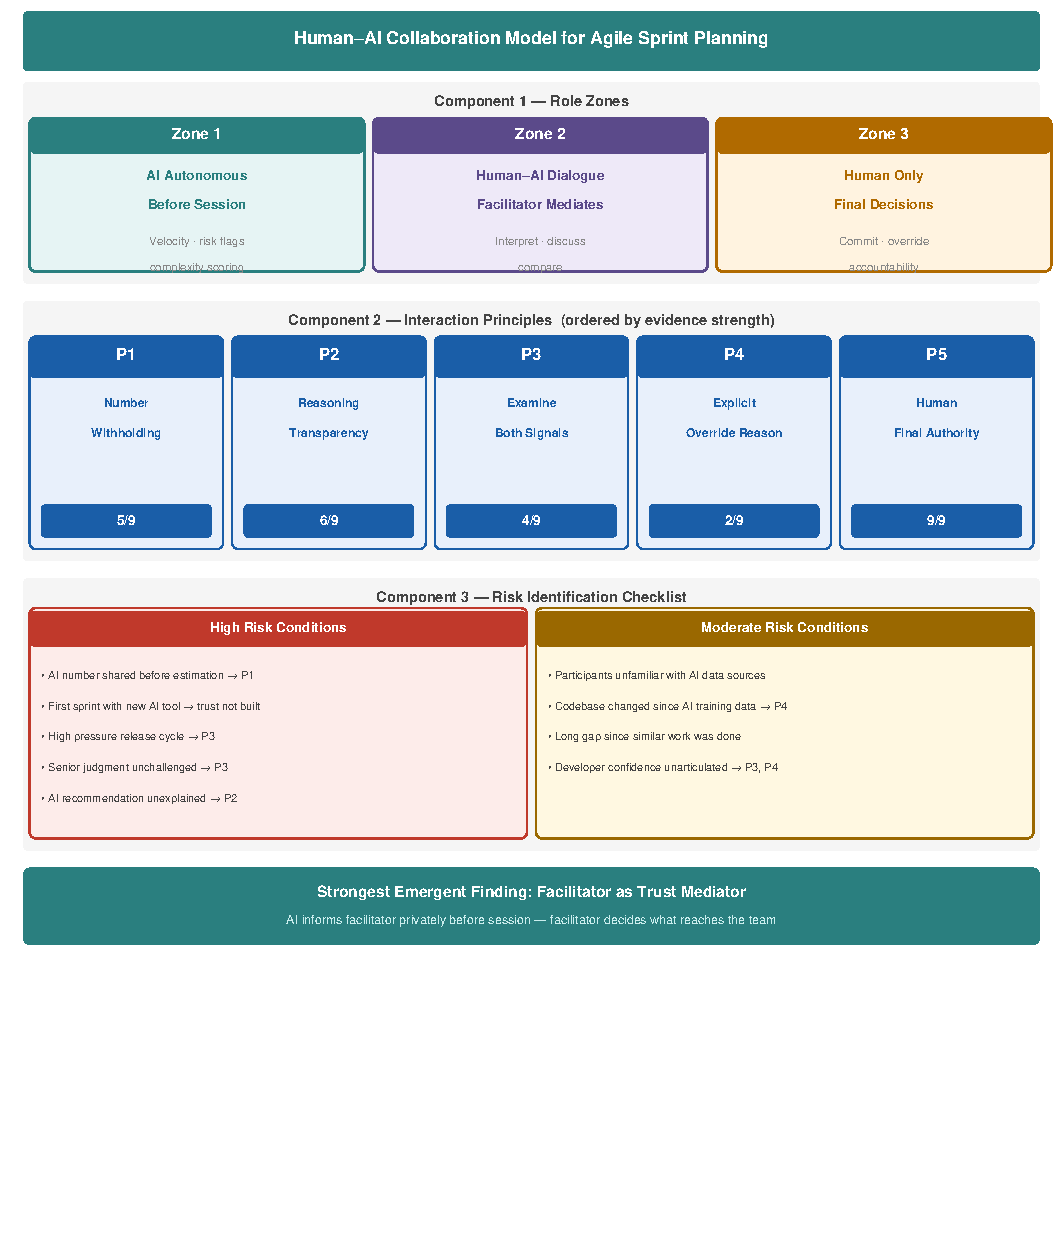
\includegraphics[width=0.95\textwidth]{model_figure.pdf}
\caption{Process map for Human-AI collaboration in Agile sprint planning. Before planning, the facilitator uses Zone 1 to review AI analysis privately. During planning, Zone 2 shows how signals can be introduced without exposing the team to an early numerical anchor. Zone 3 identifies decisions that remain human-only. The five interaction principles govern information flow between zones; the risk checklist indicates when additional safeguards are required.}
\label{fig:model}
\end{figure}

\begin{table}[htb]
\caption{Summary of model components}
\label{tab:model}
\centering
\begin{tabular}{p{3cm} p{9.5cm}}
\toprule
Component & Description \\
\midrule
Role Zone 1 & AI analytical support before session: velocity analysis, risk flagging, preliminary complexity flagging, ungrouped backlog flagging \\
Role Zone 2 & Human-AI dialogue: facilitator interprets AI tool signals, post-estimation comparison \\
Role Zone 3 & Human only: final commitment, override decisions, performance judgement \\
\midrule
Principle 1 & Withhold AI tool figure until after independent team estimation \\
Principle 2 & Require AI tool to explain reasoning basis \\
Principle 3 & Examine both AI tool and developer signals before deciding \\
Principle 4 & Require explicit concrete justification for any override \\
Principle 5 & Human final authority on all commitment decisions \\
\midrule
Risk checklist & 5 high-risk and 8 moderate-risk conditions with mapped mitigations \\
\bottomrule
\end{tabular}
\end{table}

\subsection{How the Model Answers the Research Questions}

The three components of the model map directly onto the four research questions. RQ1a asked how practitioners describe anchoring and algorithm aversion risk as affecting reasoning in AI-assisted sprint planning. The model answers this through the risk identification checklist, which specifies thirteen conditions under which these patterns are most likely to be described as problematic. Five high-risk conditions address the most acute risks; eight moderate-risk conditions address additional contextual factors identified by participants.

RQ1b asked how practitioners describe these patterns as manifesting. Anchoring is described as manifesting through reference-point adjustment, which Principle~1 (number withholding) is designed to reduce the risk of. The dismissal-without-engagement pattern is described as manifesting through developer authority assertion, which Principle~3 (examine both signals) and Principle~4 (explicit override justification) counter by requiring articulated evidence.

RQ2 asked how practitioners describe trust calibration. Zone~2 positions the facilitator as the trust mediator between AI output and team reasoning. Principle~2 requires the AI tool to explain its reasoning basis, which is the precondition for calibration identified by Lee and See~\cite{lee2004trust}.

RQ3 asked what practitioner-informed principles can be proposed for structuring Human-AI collaboration in sprint planning while preserving human oversight. The model is the direct answer: five interaction principles, three role zones, and thirteen risk conditions derived from practitioner accounts and grounded in the HACO taxonomy and Lee and See's calibrated trust theory. Team-level effectiveness, collective acceptance and behavioural outcomes remain untested and require future team-level observation or intervention studies.

\subsection{Practical Application in Sprint Planning}

The model is designed to be used by a Scrum Master or sprint planning facilitator. The following describes how the three components work together in a real planning session.

\textbf{Before the session.} The Scrum Master reviews the AI tool's output privately, without sharing it with the team. Using the risk checklist, they assess whether any high-risk or moderate-risk conditions apply. Based on this assessment, they decide which AI signals are worth raising during the session and how to frame them. The AI tool's specific numerical recommendations are not brought into the room at this stage.

\textbf{During the session.} The team estimates independently using their usual process, without any AI figure in the room. This preserves independent team estimation and prevents number-first contamination. Only after the team has committed to their estimates does the facilitator introduce any relevant AI signals, framing them as data points to consider rather than recommendations to accept or reject. If the AI tool flagged a specific story as high risk, the facilitator uses Principle~3 (examine both signals) to surface the disagreement and ask the assigned developer to articulate why the story differs from the historical patterns the AI tool is drawing on. If the team decides to override the AI tool's signal, Principle~4 requires them to state a concrete reason.

\textbf{After the session.} The facilitator compares the team's committed sprint scope against the AI tool's recommendations and notes any significant gaps. Over time, tracking whether the AI tool was right in cases where the team overrode it builds the track record that enables calibrated trust.

The model does not prescribe every facilitation decision. It sets the structural conditions under which Human-AI collaboration is less likely to produce anchoring or dismissal-without-engagement patterns, while leaving facilitation judgement where it belongs: with the experienced practitioner in the room.

\chapter{Discussion}
\label{chp:discussion}

\section{Interpretation of Findings}

\subsection{Anchoring risk in AI-assisted sprint planning}

Prior work has documented anchoring as a general pattern in software estimation~\cite{mohanani2018cognitive}. What this study adds is practitioner accounts grounded at the specific moment of interaction: the point at which an AI tool's figure enters a planning room. The distinction between a figure treated as a reference and one treated as evidence was articulated most precisely by P6 in response to Vignette A and is the practical crux of the anchoring problem in AI-assisted planning.

The number-withholding approach is one of the most consistent findings of this study. It was described independently by five participants, two of whom connected it explicitly to real past experience of anchoring effects. This makes it stronger evidence than a theoretically derived prescription would be, though it should be noted that the primary source for most of these descriptions was Vignette A responses rather than direct observation of real practice.

The finding also connects to Drury-Grogan and O'Dwyer's~\cite{drury2013investigation} observation that time pressure increases heuristic reasoning. When a number is already in the room, time-pressured teams are more likely to adjust from it rather than form independent judgements.

\subsection{Algorithm aversion risk patterns in context}

The dismissal-without-engagement reasoning observed in vignette responses is more varied than Dietvorst et al.'s~\cite{dietvorst2015algorithm} original characterisation of algorithm aversion. Most participants did not describe blanket rejection but contextual scepticism, questioning whether the AI tool's historical pattern was applicable to the current situation. As noted in the methods section, this study examines reasoning patterns related to algorithm aversion risk rather than measuring algorithm aversion in the strict experimental sense.

This likely reflects the specific population. All participants were experienced practitioners with more than five years in Agile roles. Experienced practitioners may have developed more sophisticated approaches to evaluating AI recommendations precisely because they have enough domain knowledge to interrogate the tool's evidence base.

The clearest evidence of dismissal without engagement in this study comes from P4's recounted real incident: the developer asserted familiarity with the codebase, the team sided with the developer without examining the AI tool's historical evidence, and the story ran approximately 45\% over estimate. P4 subsequently changed their facilitation approach by examining the historical basis of AI warnings before accepting or dismissing them. No participant directly demonstrated B1 in their own Vignette B response; most participants instead described calibrated scepticism.

\subsection{Trust calibration}

The consistent identification of transparency of reasoning as a key trust condition connects directly to Lee and See's~\cite{lee2004trust} definition of appropriate reliance as trust proportional to a tool's actual capabilities. Practitioners cannot calibrate reliance to actual capability if they cannot see the basis for a recommendation. Transparency is the precondition for calibration.

The level of transparency participants described as sufficient was quite modest: one or two sentences. The design requirement is not complex explainability infrastructure but minimal traceability.

The facilitator-as-mediator pattern connects to Emmanouilidis et al.'s~\cite{emmanouilidis2025co} observation that interaction protocol design, not AI tool accuracy, determines whether collaboration produces better outcomes. The number-withholding practice is exactly such a protocol: a deliberate choice about when and how AI tool output enters the planning room.

\subsection{Implications for AI tool design}

The findings suggest a hypothesis for future investigation: AI sprint planning tools that present numerical recommendations before independent team estimation may inadvertently increase anchoring risk, regardless of their predictive accuracy. This claim was not directly tested in this study (no tool interaction was directly observed) and should be understood as a hypothesis generated by practitioner accounts and vignette reasoning, requiring empirical validation. With that caveat, the findings do suggest that the primary limitation of existing tools may not be predictive accuracy but the interaction design through which recommendations reach the team.

\section{The Conceptual Model in Context}

\subsection{How the model relates to HACO}

The conceptual model builds on the HACO taxonomy~\cite{dubey2020haco} but differs from it in important ways. HACO organises Human-AI teaming across four meta-dimensions: task characteristics, learning paradigm, teaming characteristics, and trust. All four were used as a coding lens during Phase~B of the thematic analysis. Three of the four produced model components with sufficient empirical grounding.

Task characteristics shaped the role zone definitions. Teaming characteristics fed into the interaction principles, particularly the facilitator-as-mediator pattern, the examine-both-signals principle, and the explicit override justification principle. The trust dimension informed the transparency requirement and the risk checklist conditions.

The learning paradigm dimension did not produce a standalone model component. Participants described human learning from experience: P4's account of updating facilitation practice after the AI tool proved correct is the clearest example. However, the data did not surface consistent themes around how AI tools themselves learn or adapt within sprint planning contexts. Three factors likely explain this: the interview format captures a single point in time; current AI planning tools do not visibly adapt their recommendations in ways practitioners notice; and the interview guide did not include a direct question about AI tool adaptation.

The model goes beyond what HACO alone could provide because it is grounded in empirical data from a specific context. HACO identifies calibrated trust as a desirable state but does not specify what causes practitioners to drift toward anchoring or dismissal-without-engagement patterns, or what safeguards prevent it. Our model addresses that gap for the sprint planning context.

\subsection{Relationship to Lee and See's trust theory}

Lee and See's~\cite{lee2004trust} definition of calibrated trust provides the theoretical foundation for the model's trust-related principles. Principle~2, the reasoning transparency requirement, directly operationalises calibrated trust. Principle~1, number withholding, addresses a condition that Lee and See's theory implies but does not specify: when an AI tool recommendation enters the room before independent estimation, the conditions for calibrated trust are undermined regardless of how transparent the tool is. Number withholding creates the precondition for calibrated trust by ensuring team reasoning forms independently before AI tool output is introduced.

\subsection{Validation findings}

The second structured validation round was conducted via email with P6, P8, and P4 during August--September 2026. Full responses are in Appendix~\ref{app:validation}. The following summarises the key findings from this round.

All three participants considered the zone structure plausible, although its alignment with their current practice varied. P6 noted that ``before the session'' in Zone 1 must mean truly before, not merely silent in the room, since tools that are technically quiet but still visible during refinement can still be referenced live. P8 raised a related distinction between ambient tools (visible in Jira but not actively pushing a number) and actively-pushing tools, suggesting the model could make this distinction more explicit. P4 offered an honest assessment: Zone 1 describes where he aspires to be more than where he currently is, since he still shares the LinearB velocity chart directly with his team at the start of planning and has observed it anchoring them.

On the interaction principles, all three confirmed number withholding as the most important. P8 confirmed this from direct experience: he tested the opposite early on, shared the number before estimation, and watched estimates cluster around it; he stopped doing that and estimation became noticeably more independent. P6 raised a nuance on human final authority: it is not just the commitment that must stay human but the reasoning behind the commitment: if the AI shaped the reasoning, the team has not really made the call even if they technically said yes. P4 confirmed the examine-both-signals principle from a real incident where not doing this cost his team; a senior developer's assumption about the data model had changed, nobody pushed back due to his seniority, and the story ran over.

P6 identified unacknowledged trust erosion as a risk not previously in the checklist: a tool can quietly lose credibility through repeated misses that go unremarked, without a formal decision to stop trusting it. P8 identified short-term availability blind spots as distinct from structural team composition change: one-off situations such as a team member on leave or a mid-sprint disruption are not visible to the AI tool and can make its recommendations systematically wrong for that period. Both were added to the checklist as moderate risk items 12 and 13 respectively.

Both P6 and P8 independently raised a concern about checklist item 9 wording: confidence itself is not the risk; the risk is confidence that falls apart when asked to articulate its basis. The wording was updated to ``developer override asserted without articulated basis'' to reflect this.

P4 provided the most frank assessment of all three validators: ``I don't think I'm the cleanest example to build the ideal version of this model around. A lot of what I've told you is tension I haven't sorted out yet {[}\ldots{]}.'' This candid response is noted as useful context for interpreting the model's practical scope: the principles describe a standard practitioners are working toward, not one all experienced Scrum Masters have fully implemented.

\subsection{Scope and generalisability}

The model applies to Agile sprint planning. Whether the principles generalise to other Agile ceremonies is an empirical question this study cannot answer. Some principles, particularly human final authority and reasoning transparency, are likely relevant in any Human-AI decision-making context. Others, particularly number withholding, are specific to estimation contexts where a figure can become an anchor.

An important scope constraint concerns the facilitation role. Five of nine participants were Scrum Masters, and the facilitator-as-mediator finding maps directly onto the Scrum Master role. For teams without a dedicated Scrum Master (flat teams, self-organising teams, or teams where sprint planning is run by a rotating lead), the model in its current form may not be directly applicable. This is documented as a limitation and direction for future work.

\section{Convergence of Evidence Across Interview Parts}

Three types of evidence were collected across the three interview parts, and their convergence strengthens the analytical claims where it occurs and reveals their limits where it does not.

For the number-withholding practice, Part 2 vignette responses (P3, P4, P6, P7, P8) converge on the same practice. P7 connected their vignette response to a real anchoring incident; P8 reported implementing number withholding as an ongoing practice. This distinction matters: P7's account describes learning from experience and intention, while P8's describes actual implementation. This convergence across evidence types is the strongest support available within this study's design and elevates number withholding from a hypothetical prescription to a practice with some real-world grounding.

For the facilitator-as-mediator finding, the evidence comes primarily from Part 3 self-report, which carries Nisbett and Wilson's~\cite{nisbett1977telling} caveat about self-report validity. The finding is supported by five participants independently describing the same setup, but all five are describing what they believe should happen or aspire to do, and P4 confirmed during the validation round that he does not yet fully live this principle in practice. The finding is therefore presented as an aspirational model with strong practitioner endorsement rather than as a description of current widespread practice.

For the dismissal-without-engagement pattern, the clearest evidence comes from P4's real incident recounted during Vignette B follow-up questions. No participant directly demonstrated B1 in their own vignette response. The pattern is therefore supported by one recounted real incident, which is a weaker evidential base than number withholding.

\section{The Role of Practitioner Experience in Bias Calibration}

The evidence did not support a clear directional relationship between practitioner experience, AI-tool exposure and bias calibration. P2, who reported no direct AI planning-tool experience, provided the clearest anchoring response. However, the clearest dismissal-without-engagement evidence came from a real incident recounted by P4, who had direct AI-tool experience. More experienced participants also described several sophisticated safeguards, including number withholding and the examine-both-signals approach, but the small and uneven sample does not support comparative conclusions about the effect of experience on bias calibration.

\section{Limitations}

This study produced a conceptual model, not a deployable tool or a statistically generalisable theory. The study is limited by its small sample size (n=9), which constrains generalisability beyond the studied context. The findings should therefore be interpreted as exploratory rather than representative of the broader Agile practitioner population~\cite{creswell2013}.

The primary data source for most findings is vignette responses and Part 3 self-report. Vignette responses represent hypothetical reasoning about a described scenario. Whether participants' described practices match their actual behaviour in live planning sessions cannot be confirmed from this data alone. This is a structural limitation of the research design.

The model's practical credibility was assessed through structured walkthroughs with three original participants. The walkthroughs confirmed the model's plausibility and produced three refinements incorporated into this version. The model's generalisability beyond the studied context remains a limitation regardless of this assessment.

The consent information sheet disclosed that the study examined cognitive bias patterns and trust calibration in Human-AI collaboration. This disclosure may have primed participant responses, particularly in the vignette sections, as participants were aware of the study's focus before responding to the scenarios. This is acknowledged as a limitation of the study design that cannot be retroactively addressed.

\section{Ethical and Societal Considerations}

The most significant ethical concern is \textit{deskilling}. As AI tools take on more analytical work in sprint planning, practitioners risk losing competence in independent reasoning. Research on automation has documented this pattern~\cite{parasuraman2010complacency}. The model includes explicit checkpoints (the examine-both-signals principle and the explicit override justification requirement) that require active human engagement rather than passive acceptance.

All participant identities and organisations were fully anonymised. No sprint records, backlog items, or organisational data were collected. Research instruments, the anonymised codebook, data documentation, and handwritten analysis notes are available at \url{https://doi.org/10.5281/zenodo.20529721}. Full interview transcripts will not be publicly released due to participant confidentiality commitments, but are available to the thesis supervisor and examiner upon request.

\section{Implications for Research}

This study raises several directions for future empirical work. First, the facilitator-as-mediator pattern was identified through practitioner accounts and vignette responses, not direct observation. Future research should investigate whether teams whose facilitators withhold AI figures before estimation produce less anchored commitments than teams where figures are shared directly. An observational or quasi-experimental design comparing these two conditions would provide evidence that the current study cannot.

Second, the trust calibration conditions identified here (transparency, track record, and contextual applicability) were described by practitioners in Part 3 self-report. Whether these conditions actually predict reliance behaviour in practice is an open empirical question. Longitudinal studies tracking how trust in AI planning tools develops over multiple sprints would be better positioned to examine trust calibration as a dynamic process rather than a stated preference~\cite{lee2004trust}.

Third, the learning paradigm dimension of HACO produced no model component in this study. Future research investigating how AI planning tools learn from team feedback across sprints, and how practitioners perceive and respond to that adaptation, would address a gap this study could not fill with single-session interviews.

Fourth, the possible relationship between practitioner experience, AI-tool exposure and bias calibration warrants direct investigation. This study did not establish a directional relationship between these factors. A comparative study involving novice and experienced Scrum Masters could examine whether experience affects recognition of anchoring and dismissal risks or the application of the proposed safeguards.

\section{Implications for Practice}

For Scrum Masters and sprint planning facilitators, the most immediately applicable finding is the number-withholding principle: reviewing AI tool recommendations privately before the session and keeping specific figures from the team until after independent estimation. Five participants converged on this practice in their responses, with two connecting it to direct real-world experience of anchoring effects. It requires no new tools or organisational change, only a deliberate facilitation decision about when AI output enters the room.

For organisations introducing AI planning tools, the transparency finding has direct design implications. Practitioners described needing only one or two sentences of explanation to enable calibrated trust: which specific past stories the AI is drawing on, and what went wrong with them. Tools that surface this minimal traceability are likely to produce better practitioner engagement than tools that output only a figure. The barrier to enabling calibrated trust through transparency is low.

For teams in the first sprint with a new AI planning tool, the risk checklist identifies this as a high-risk condition. Organisations should treat the first several sprints as a trust calibration period, tracking cases where the team overrides the AI tool and whether the tool was subsequently found to be right. Building this track record deliberately may support more calibrated reliance over time~\cite{lee2004trust}.

The validation round raised a practical note about unacknowledged trust erosion (checklist item 12): trust can degrade quietly through repeated misses that go unremarked, without anyone deciding to stop trusting the tool. Organisations should build explicit periodic review of AI tool accuracy into their retrospective process, rather than assuming calibration happens automatically.


\chapter{Conclusions and Future Work}
\label{chp:conclusions}

\section{Answers to Research Questions}

\textbf{RQ1a: How do practitioners describe anchoring bias and patterns associated with algorithm aversion risk as affecting reasoning in Agile sprint planning when AI recommendations are introduced?}

Anchoring risk was the concern raised most consistently and independently across the study. Five of nine participants described number-first contamination as a relevant risk to practitioner reasoning, with two connecting it explicitly to direct first-hand experience in real planning sessions. Patterns associated with algorithm aversion risk were described in a more varied form than prior literature suggests: experienced practitioners described calibrated scepticism rather than blanket rejection, distinguishing between legitimate dismissal based on identifiable contextual differences and unjustified dismissal through assertion of domain authority without evidence.

\textbf{RQ1b: How do practitioners describe these bias patterns as manifesting in reasoning during AI-assisted planning scenarios?}

Anchoring risk is described as manifesting through reference-point adjustment: when an AI tool figure is shared before independent estimation, reasoning adjusts from it rather than forming an independent judgement. The dismissal-without-engagement pattern is described as manifesting through developer authority assertion, invoking domain expertise to dismiss an AI tool flag without articulating a specific basis. Experienced facilitators described explicit practices to counter both: number withholding for anchoring and examine-both-signals facilitation for the dismissal pattern.

\textbf{RQ2: How do Agile practitioners describe trust calibration in AI tools when delegating planning tasks, and what conditions do they identify as leading to overtrust or distrust?}

Trust calibration was described as shaped by three conditions practitioners identified: transparency of AI tool reasoning, track record over time, and contextual applicability of historical patterns. A recurring pattern across Part 3 responses was that experienced practitioners independently converged on a facilitator-as-mediator model, in which the AI tool informs the facilitator privately before the session and the facilitator decides what to bring to the team and how to frame it.

\textbf{RQ3: What practitioner-informed principles can be proposed for structuring Human-AI collaboration in Agile sprint planning while preserving human oversight?}

The conceptual model specifies five interaction principles: (1) withhold AI tool-suggested figures until after independent team estimation; (2) require the AI tool to explain the basis for its recommendations; (3) examine both AI tool and developer signals before deciding; (4) require explicit concrete justification for any override; and (5) maintain human final authority on all commitment decisions. These are accompanied by three-zone role definitions and a thirteen-condition risk identification checklist, expanded from the original eleven conditions following the second validation round.

\section{Contributions}

This thesis makes two contributions to the Human-AI collaboration literature in software engineering.

The first is an \textbf{empirical contribution}: interview data from nine Agile practitioners documenting how practitioners describe anchoring and algorithm aversion risk patterns as manifesting in reasoning about AI tool recommendations during sprint planning, and the conditions practitioners describe as shaping trust and appropriate reliance in that context. Based on the reviewed literature, no prior study was found combining practitioner account data on cognitive bias and trust in AI-assisted sprint planning in a single study. The interview guide, consent information sheet, anonymised codebook, and data documentation are available at \url{https://doi.org/10.5281/zenodo.20529721}.

The second is the \textbf{conceptual model}: a structured specification of role definitions, interaction principles, and risk conditions for Human-AI collaboration in Agile sprint planning, grounded in practitioner accounts. A prominent empirical pattern in this study was the facilitator-as-mediator configuration, described by five participants who converged on the same facilitator-as-mediator interaction structure. This finding is consistent with prior work highlighting the importance of facilitator mediation in AI-assisted Agile meetings~\cite{cabrero2024exploring}, while this study extends that idea by specifying how practitioners described mediation in relation to independent estimation, anchoring risk, and human oversight. The model as a whole is a design artefact that practitioners and researchers can use as a reference when structuring Human-AI collaboration in sprint planning contexts.

\section{Future Work}

The model is grounded in individual practitioner accounts and has not been tested at the team level. Testing the model in real sprint planning sessions with full teams is the natural next step.

Future work could extend the model to other Agile ceremonies and investigate whether the same bias patterns appear in other AI-assisted decision-making contexts in software engineering.

The facilitator-as-mediator finding raises a practical question this study could not answer: what happens in teams without a dedicated Scrum Master? The model's effectiveness depends on facilitation competence, which may limit its applicability in flat or self-organising teams. Investigating how the principles can be operationalised without a dedicated facilitator is a relevant extension.

The learning paradigm dimension of HACO did not produce a standalone model component in this study. Future work investigating how AI planning tools learn from team behaviour across sprints, and how practitioners respond to that adaptation, would address this gap directly.

Finally, the transparency finding (that practitioners described needing only one or two sentences of explanation to enable calibrated trust) has direct implications for AI tool design. Future work could investigate whether building minimal traceability into AI planning tools measurably improves trust calibration and reduces both anchoring and dismissal-without-engagement patterns in practice.


\bibliographystyle{IEEEtranS}
\bibliography{references}


\appendix

\chapter{Interview Guide}
\label{app:interview}

\section*{Part 1: Background (approximately 8 minutes)}

\begin{enumerate}
  \item Can you tell me about your current role and how long you have been working in Agile teams?
  \item Walk me through how your team runs a typical sprint planning session: who is involved, how long it takes, and how you reach the final commitment.
  \item What are the most common difficulties your team faces during sprint planning?
  \item Does your team use any AI tools to support sprint planning decisions? If yes, what does that look like in practice?\\
  \textit{[If no AI experience: ``Has AI come up in any conversation about your planning process, even if not adopted yet?'']}
\end{enumerate}

\section*{Part 2: Vignette Scenarios (approximately 12 minutes)}

\textit{Do not tell participants what you are looking for. Read each scenario naturally and let them talk.}

\subsection*{Vignette A: Anchoring Bias}

\textit{Read aloud:} ``Your team is in sprint planning. An AI tool has analysed your backlog and past velocity data and recommends committing to 42 story points this sprint. Your team's average over the last five sprints has been 34 points. The AI tool explains that three similar stories were completed faster than expected recently, which is why it suggests a higher commitment.''

\begin{enumerate}
  \setcounter{enumi}{4}
  \item What would you and your team do with this recommendation? Accept it, adjust it, or ignore it? Walk me through your thinking.
  \item What information would you need before feeling confident making a decision here?
  \item If your team's discussion started revolving around the number 42 rather than your usual 34, would that concern you? Why or why not?
  \item Who would have the most influence over the final decision: the AI tool recommendation, the Scrum Master, the developers, or someone else?
\end{enumerate}

\subsection*{Vignette B: Patterns Associated with Algorithm Aversion Risk}

\textit{Read aloud:} ``The same AI tool flags that a story your team has already agreed to include this sprint will likely take 60\% longer than estimated, based on similar past stories. The developer assigned to that story disagrees. They say they know this part of the codebase well and are confident in the original estimate.''

\begin{enumerate}
  \setcounter{enumi}{8}
  \item How would your team handle this? Side with the AI tool, the developer, or find a middle ground?
  \item Have you ever been in a situation where a tool's recommendation conflicted with a team member's judgement? What happened?
  \item What would make you more willing to trust the AI tool's warning in this case?
\end{enumerate}

\section*{Part 3: Trust (approximately 10 minutes)}

\begin{enumerate}
  \setcounter{enumi}{11}
  \item When you receive a recommendation from an AI tool during planning, what makes you trust it enough to act on it?
  \item Can you describe a specific time when you trusted an AI tool recommendation and it turned out to be wrong? How did that change how you used the tool afterwards?\\
  \textit{[If no AI experience: ``What would make you trust or distrust an AI tool recommendation? What would it need to show you?'']}
  \item How important is it that an AI tool explains its reasoning, not just the output but why it made that recommendation?
  \item Is there any planning decision you would never delegate to an AI tool, no matter how accurate it was? What and why?
  \item What would an AI tool need to show you, in terms of transparency, track record, or explanation, before you felt comfortable letting it handle a planning decision without your direct review?
  \item If you imagine sprint planning where AI tools and humans work together well, what does that actually look like? Who does what?
\end{enumerate}

\section*{Closing}

\begin{enumerate}
  \setcounter{enumi}{17}
  \item Is there anything about AI in sprint planning that you think researchers typically miss or get wrong?
\end{enumerate}

\textit{Note: the first interview (P5, 18 April 2026) deviated from this sequence. The Part 3 trust questions were asked before the vignettes, and only Vignette A was administered. For P3 (3 May 2026), who had no direct AI tool experience, the vignette wording was adapted to a third-person framing at the interviewer's discretion.}


\chapter{Codebook}
\label{app:codebook}

The codebook is organised into three groups corresponding to the three main analytical themes that emerged from the data. Group~A covers anchoring codes, capturing the mechanism of number-first contamination, how it is described as manifesting in reasoning, and the safeguard practitioners described in response. Group~B covers algorithm aversion risk pattern codes, capturing the full spectrum from unjustified rejection to calibrated scepticism. Group~C covers trust calibration codes, capturing what drives trust up and down and how the facilitator-as-mediator model works in practice.

\section*{Anchoring codes}

\textbf{A1: Number-first contamination.} Participant describes the risk of an AI tool figure shared before independent team estimation shaping subsequent reasoning, or participant's own vignette reasoning begins from the AI tool's figure.

\textbf{A2: Reference-point adjustment.} Participant reasons from the AI tool's figure rather than forming an independent judgement in the vignette response.

\textbf{A3: Number withholding (safeguard).} Participant describes a deliberate practice of keeping the AI tool's figure private until after team estimation, whether as hypothetical vignette response or described real practice.

\section*{Algorithm aversion risk pattern codes}

\textbf{B1: Developer authority assertion.} Coded when a developer or participant invokes domain expertise to dismiss an AI tool flag without articulating a specific, concrete basis for the dismissal.

\textbf{B2: Examine both signals (safeguard).} Facilitator describes requiring both AI tool and developer to articulate their basis before the team decides.

\textbf{B3: Pattern match scepticism.} Participant questions whether the AI tool's historical patterns apply to the current context.

\textbf{B4: Legitimate contextual dismissal.} Override described as based on a concrete identifiable reason that the AI tool's evidence does not apply.

\section*{Trust calibration codes}

\textbf{C1: Transparency drives trust.} Participant describes trust increasing when the AI tool explains the basis for its recommendation.

\textbf{C2: Track record drives trust.} Trust described as updated by past experience of AI tool accuracy or inaccuracy.

\textbf{C3: Human final authority.} Final commitment decision described as needing to remain with the team regardless of AI tool capability.

\textbf{C4: Facilitator as mediator.} Participant describes AI tool informing facilitator before session; facilitator decides what to bring and how to frame it.

\textbf{C5: Contextual applicability assessment.} Trust described as calibrated by assessing whether AI tool patterns apply to current specific conditions.


\chapter{Validation Walkthrough Materials}
\label{app:validation}

\section*{Context and participant selection}

Two validation rounds were conducted. An initial informal walkthrough was conducted with P6, P7, and P8 via message exchange in May 2026. These responses were informal and preliminary, and a complete written record is not available. Following examiner review, a second structured validation round was conducted via email during August--September 2026 to produce a verifiable written record of participant feedback.

For the second round, P7 was unavailable despite multiple contact attempts. P4 was invited as a replacement. P4 was selected because P4 provided one of the richest interviews in the study, including a real incident where dismissing an AI tool warning led to a story running approximately 45\% over estimate, and has direct ongoing experience with an AI planning tool in practice.

All participant identities are anonymised throughout this appendix. Email signatures in the responses below have been replaced with participant codes to maintain consistency with the anonymisation commitments made in the consent information sheet.

\section*{Outreach message sent to P6, P8, and P4 (second validation round)}

The following message was sent to the three participants via email in August 2026. Each participant had completed a full interview and was familiar with the research context.

\begin{quote}
Hi [name], hope you are doing well.

We are revising our thesis on Human-AI collaboration in sprint planning and would really value your feedback on the model we developed from the interviews. We are reaching out again because we want to make sure we have a clear written record of participant responses to the model --- the examiner reviewing our thesis has asked us to be more transparent about how the validation was conducted.

Here is a summary of the model as it stands now:

\textbf{Role Zones.} Zone 1: AI does the data work privately before the session --- velocity trends, risk flagging, complexity flagging, backlog description gaps. It stays outside the planning room. Zone 2: The Scrum Master or facilitator reviews AI output privately and decides what signals are worth bringing into the session and how to frame them. Zone 3: Human only --- final sprint commitment, override decisions, performance judgements.

\textbf{Interaction Principles.} (1) Number withholding: the AI-suggested figure is never shared with the team before they estimate independently. (2) Reasoning transparency: the AI must explain which past stories it is drawing on and why, in plain language. (3) Examine both signals: when the AI and a developer disagree, both must articulate their basis before a decision is made. (4) Explicit override justification: any override of an AI recommendation must state a concrete, specific reason. (5) Human final authority: the final sprint commitment always belongs to the team.

\textbf{Risk Checklist.} High risk: AI figure shared before team estimates, first sprint with new tool, high-pressure release cycle, senior judgement unchallenged, AI recommendation with no explanation. Moderate risk: team unfamiliar with AI data sources, significant codebase changes, long gap since similar work, developer override without articulated basis, significant team composition change, sprint inertia from recent good run.

Three questions: (1) Looking at the three zones --- does this reflect how you think AI should be involved in sprint planning? Anything missing or unrealistic? (2) Looking at the five principles --- any you would not follow in practice? Any missing? (3) Looking at the risk checklist --- does this match your experience? Anything to add or remove?

Please reply by email at your convenience. We really appreciate your time.
\end{quote}

\section*{P6 response (Scrum Master, 8+ years experience)}

The following is the full email response received from P6.

\begin{quote}
Hi Mihir and Yash,

Sorry for the late response, been busy with work. Thanks for sending this over, good to see it pulled together like this.

On the zones, yeah, it matches how I already think about it. AI doing prep work before the session, staying out of the room, and me deciding what's worth surfacing, that's basically what I already do manually with burn-down data and backlog signals, so no objection there. If anything I'd push you to be explicit in Zone 1 that `before the session' really means before, not just `not speaking directly to the team', I've seen tools that technically stay silent in the room but still get referenced live, which defeats the purpose.

On the principles, mostly agree, a few notes:

Number withholding: fully agree, this is the one I care about most. A number shown before independent estimation just becomes the anchor whether you want it to or not.

Reasoning transparency: agree in spirit, but be careful how you word this one. I don't want maximal explanation, I want enough. A sentence or two on which stories it's drawing from and why is useful. Anything more turns planning into a model-debugging session. As written, ``must explain which stories it is drawing on and why'' is fine actually. Just don't let it expand into more than that.

Examining both signals: agree this is basically my code-familiarity scenario. The developer should have to walk through what makes their reading different, not just assert confidence.

Explicit override justification: agree.

Human final authority: agree, and I'd go slightly further than how you've worded it. It's not just the commitment that needs to stay human, it's the reasoning behind the commitment. If the AI shaped the reasoning, the team hasn't really made the call even if they technically said yes to it.

The risk checklist matches most of what I've actually seen. One thing I'd add that isn't on there: the risk isn't always acute. Sometimes a tool just quietly loses credibility and people stop looking at it without ever deciding to stop trusting it, that happened with a burn-down tool on my team. Might be worth adding something like ``unacknowledged trust erosion'' or similar to moderate risk, separate from ``unchallenged senior judgement,'' which is a different failure mode.

Also, I'd want to be careful putting ``unarticulated developer confidence'' as moderate risk. Confidence itself isn't the risk in my experience, it's confidence that can't be articulated when asked. Might be worth tightening the wording so it's not read as ``developers being confident is inherently risky.''

Otherwise this is solid. Happy to jump on a call if it's faster than email.

Best regards,
[P6]
\end{quote}

\section*{P8 response (Scrum Master, 6+ years experience)}

The following is the full email response received from P8.

\begin{quote}
Hi Mihir and Yash,

This is genuinely well put together, thanks for taking the time to write it up.

Starting with the zones, this is basically how I already work. I sit on the capacity plugin's number and only check it against the team's total privately, after the fact, so the Zone 1 to Zone 2 handoff is pretty much my routine. One small thing though: my backlog scoring tool is actually visible the whole time during refinement and planning, it's just sitting in the Jira view rather than being announced. So it's not quite ``never speaks to the team'', it's more like it's ambient rather than active. Might be worth drawing that distinction somewhere, because I'd treat a tool that's just sitting there differently from one that's pushing a number into the conversation, even if neither one is technically ``speaking.''

I have a few thoughts about the Interaction principles. Number withholding I'm fully behind, I actually tested the opposite early on, shared the number before estimation, and watched everyone's guesses cluster right around it. Stopped doing that and things got noticeably more honest. I'd leave that one exactly as is.

Reasoning transparency I agree with too, but I'd push it slightly further than ``must explain.'' For me the real test is whether I can turn the explanation into something plain enough to say out loud to the team. If I can't translate it, it doesn't matter that the tool technically gave a reason, I'm not bringing it in. Might be worth folding that into the wording somehow.

Examine both signals, this is close to how I already handle the code-familiarity situation. I get the developer to point to something specific rather than just asserting they know the area, and I also check what the tool's actually comparing against, because sometimes it's matching against stories from before a refactor and that's not really the same codebase anymore.

Explicit override justification, agreed. The thing I'd add is that I try to hold both sides to the same bar, if the tool's probably right and the developer's pushback is thin, I go with the tool; if the developer's got something concrete, I go with them. It's less about who's right more often and more about being consistent either way.

Human final authority, agreed. Though I'd tighten the wording a little. There's a real gap between a team saying ``we're committing to this'' and a team saying ``the tool said we had room so nobody objected.'' The second one isn't really ownership, it just looks like it until something goes wrong.

The risk checklist mostly lines up. Two things worth raising. First, ``unarticulated developer confidence'' --- but confidence itself isn't the problem, it's confidence that falls apart the moment you ask someone to explain it. Might be worth being a bit more precise there so it doesn't come across as ``confidence is bad.'' Second, I think there's something missing around short-term blind spots, someone on leave, a mid-sprint disruption, a week where the team's availability is just off. My tool has been clearly wrong specifically in those situations because it has no way to see them coming, and it burns trust fast when that happens. That's different from ``team composition change'' on your list, which reads more like a longer structural shift than a one-off gap.

One more thing, more general than a specific edit, the part of my tools that actually mattered wasn't the recommendation, it was the background pattern underneath it, which story types tend to overrun, when velocity dips and why. Honestly the recommendation itself was the least useful part of the whole thing. Might be worth pulling that apart somewhere as two different things AI can hand you, insight versus recommendation, since they carry pretty different risks.

Good luck finalizing the thesis!

Best,
[P8]
\end{quote}

\section*{P4 response (Scrum Master, 5+ years experience)}

The following is the full email response received from P4. P4 replaced P7 in this round as P7 was unavailable.

\begin{quote}
Hello Mihir and Yash,

Thanks for putting this together, it's genuinely helpful to see it laid out. Full disclosure though, a lot of this touches on stuff I still haven't really worked out in my own practice, so bear with me if some of this comes across as less settled than what you probably got from others.

I mostly agree on the role zones, but I want to be straight with you: Zone 1 describes where I'd like to be more than where I actually am. I still show the LinearB velocity chart directly to the team at the start of planning, which is really a Zone 1 tool leaking into the room rather than staying behind the scenes like the model describes. I've watched it anchor the team more than once, but I haven't actually stopped doing it. So I think the model itself is right, I'm just behind it in practice.

Same story with the principles, honestly. I agree with Number withholding more than I live it. I've got a real example where a velocity chart pushed the team toward a specific number, a 40 chart that turned into a 41-point commitment and a genuinely rough sprint. So I know the risk is real, I just haven't resolved the tension between wanting to be transparent with the data I have and knowing that showing it anchors people. If it's useful, ask me about that incident directly sometime, it's probably a better illustration of principle 1 than anything I can say in the abstract.

I'm fully behind Reasoning transparency, I won't bring something into a room I can't explain. If a developer asks why the tool flagged something and I don't have an answer, I've basically introduced an authority I can't back up, and that's worse than just not mentioning it.

I completely agree with examining both signals, and I've got a case where not doing this cost us. A developer who knew the domain well was confident based on an assumption about the data model that had actually changed, nobody on the team pushed back because he was senior, and the story ran way over. Since then I've made it a habit to actually look at what the tool's drawing on together with whoever's pushing back, rather than only doing that when there's obvious tension.

I agree with Explicit override justification too, though I'd point out the risk goes both directions. I've overridden a tool's recommendation by just not applying it, new team members had joined and the tool hadn't adjusted for that yet, and we ended up committing to a stale number anyway. That was on me, not the tool. Might be worth making sure the principle covers overriding the tool as much as overriding a person.

I fully agree on human final authority too, no hesitation here either, commitment needs to stay human.

A lot of the risk checklist matches what I've actually been through. Two thoughts: I'd add something like a facilitator presenting raw data without framing it, since that's exactly what caused my anchoring problem, and it's slightly different from an AI number being shared early, because in my case it wasn't the AI's number at all, it was context I chose to put in front of people that ended up doing the same thing. And team composition change, that one's real for me too, I've got a direct example of new hires and a stale velocity number causing exactly the kind of miss you'd expect.

One thing I want to say plainly, in case it's useful context for you: I don't think I'm the cleanest example to build the ideal version of this model around. A lot of what I've told you is tension I haven't sorted out yet, than something that works. If that's actually useful for showing where the principles get hard to live up to, great, use it. I just didn't want it to read as more settled than it is.

Kind regards,
[P4]
\end{quote}

\noindent Note: Two checklist items were added to the model following this second validation round. Item 12 (unacknowledged trust erosion) was raised by P6. Item 13 (short-term availability blind spots) was raised by P8. The wording of item 9 was also updated from ``developer confidence without articulated basis'' to ``developer override asserted without articulated basis'' following consistent feedback from both P6 and P8 that confidence itself is not the risk.


\clearpage
{\pagestyle{empty}
\changepage{3cm}{1cm}{-0.5cm}{-0.5cm}{}{-1.5cm}{}{}{}
\vspace*{\fill}
\center
{\bthcsnotextlogo{3cm}}
\\
\noindent\makebox[\linewidth]{\rule{\textwidth}{1pt}}
Faculty of \faculty, Blekinge Institute of Technology, 371 79 Karlskrona, Sweden
}


\end{document}